\documentclass[msc,numbers]{coppe}
\usepackage[utf8]{inputenc}
\usepackage{amsmath,amssymb, amsfonts}
\usepackage{multirow}
\usepackage{subfigure}
\usepackage{algorithmic}
\usepackage[portuguese,ruled,lined]{algorithm2e}
\usepackage{color}
\usepackage{blkarray}
\usepackage{hyperref}
\usepackage{makecell}
\usepackage{placeins}

\usepackage{empheq}
\usepackage[most]{tcolorbox}

%Definicao de qual texto será utilizado
\def\realreservoir{1}


\makelosymbols
\makeloabbreviations
\newcommand{\wbalTwo}[2][Wikimedia]{
  This is the Wikibook about LaTeX
  supported by {#1} and {#2}!}
 

\newcommand{\dx}[1][ ]{\frac{\partial {#1}}{\partial x}}
\newcommand{\dy}[1][ ]{\frac{\partial {#1}}{\partial y}}
\newcommand{\dz}[1][ ]{\frac{\partial {#1}}{\partial z}}
\newcommand{\dxi}[1][ ]{\frac{\partial {#1}}{\partial \xi}}
\newcommand{\deta}[1][ ]{\frac{\partial {#1}}{\partial \eta}}
\newcommand{\dzeta}[1][ ]{\frac{\partial {#1}}{\partial \zeta}}

\newcommand{\dxk}[1][ ]{\frac{\partial {#1}}{\partial x_k}}

\newcommand{\Tau}{\mathrm{T}}

\newcommand{\poisson}{\upsilon}

%Deslocamentos

\newcommand{\uvetor}{
\begin{bmatrix}
u_x \\ u_y \\ u_z
\end{bmatrix}
}

%Deformacoes
\newcommand{\exx}{\epsilon_{xx}}
\newcommand{\eyy}{\epsilon_{yy}}
\newcommand{\ezz}{\epsilon_{zz}}
\newcommand{\exy}{\gamma_{xy}}
\newcommand{\exz}{\gamma_{xz}}
\newcommand{\eyx}{\gamma_{yx}}
\newcommand{\eyz}{\gamma_{yz}}
\newcommand{\ezx}{\gamma_{zx}}
\newcommand{\ezy}{\gamma_{zy}}


%Definicao das tensoes efetivas
\newcommand{\sxx}{\sigma^\prime_{xx}}
\newcommand{\syy}{\sigma^\prime_{yy}}
\newcommand{\szz}{\sigma^\prime_{zz}}
\newcommand{\sxy}{\sigma^\prime_{xy}}
\newcommand{\sxz}{\sigma^\prime_{xz}}
\newcommand{\syx}{\sigma^\prime_{yx}}
\newcommand{\syz}{\sigma^\prime_{yz}}
\newcommand{\szx}{\sigma^\prime_{zx}}
\newcommand{\szy}{\sigma^\prime_{zy}}

\newcommand{\evetor}{
\begin{bmatrix}
\exx
\\
\eyy
\\
\ezz
\\
\exy
\\
\exz
\\
\eyz
\end{bmatrix}
}


% Definicao das tensoes totais
\newcommand{\stxx}{\sigma_{xx}}
\newcommand{\styy}{\sigma_{yy}}
\newcommand{\stzz}{\sigma_{zz}}
\newcommand{\stxy}{\sigma_{xy}}
\newcommand{\stxz}{\sigma_{xz}}
\newcommand{\styx}{\sigma_{yx}}
\newcommand{\styz}{\sigma_{yz}}
\newcommand{\stzx}{\sigma_{zx}}
\newcommand{\stzy}{\sigma_{zy}}

\newcommand{\stvetor}{
\begin{bmatrix}
\stxx
\\
\styy
\\
\stzz
\\
\stxy
\\
\stxz
\\
\styz
\end{bmatrix}
}

\newcommand{\stensor}{
\begin{bmatrix}
\stxx & \stxy & \stxz \\
\styx & \styy & \styz \\
\stzx & \stzy & \stzz 
\end{bmatrix}
}

\newcommand{\sstensor}{
\begin{bmatrix}
\dx[\stxx] + \dy[\stxy] + \dz[\stxz] \\
\dx[\styx] + \dy[\styy] + \dz[\styz] \\
\dx[\stzx] + \dy[\stzy] + \dz[\stzz] 
\end{bmatrix}
}

\newcommand{\Dx}{
\Delta x
}
\newcommand{\Dy}{
\Delta y
}

\newcommand{\Dz}{
\Delta z
}


%Matriz de Elasticidade
\newcommand{\elasticinv}{
\frac{1}{E}
\begin{bmatrix}
        1 & -\upsilon & -\upsilon &             0 &             0 &             0 \\ 
-\upsilon &         1 & -\upsilon &             0 &             0 &             0 \\ 
-\upsilon & -\upsilon &         1 &             0 &             0 &             0 \\ 
        0 &         0 &         0 & 2(1+\upsilon) &             0 &             0 \\ 
        0 &         0 &         0 &             0 & 2(1+\upsilon) &             0 \\ 
        0 &         0 &         0 &             0 &             0 & 2(1+\upsilon)
\end{bmatrix}
}


\newcommand{\elastic}{
\frac{E}{(1+\upsilon)(1-2\upsilon)}
\begin{bmatrix}
1 - \upsilon &     \upsilon &     \upsilon &                     0 &                     0 &                     0 \\ 
    \upsilon & 1 - \upsilon &     \upsilon &                     0 &                     0 &                     0 \\ 
    \upsilon &     \upsilon & 1 - \upsilon &                     0 &                     0 &                     0 \\ 
           0 &            0 &            0 & \frac{1-2\upsilon}{2} &                     0 &                     0 \\ 
           0 &            0 &            0 &                     0 & \frac{1-2\upsilon}{2} &                     0 \\ 
           0 &            0 &            0 &                     0 &                     0 & \frac{1-2\upsilon}{2} 
\end{bmatrix}
}


% Operador S

\newcommand{\sopwithoutb}[1][ ]{
\dx[#1] &        0 &   0      \\ 
      0 & \dy[#1]  &   0      \\ 
      0 &        0 & \dz[#1]  \\ 
\dy[#1] & \dx[#1]  &   0      \\ 
\dz[#1] &        0 & \dx[#1]  \\ 
      0 & \dz[#1]  & \dy[#1]
}

\newcommand{\sopnabla}{\nabla_S}

\newcommand{\sop}[1][ ]{
\begin{bmatrix}
\dx[#1] &        0 &   0      \\ 
      0 & \dy[#1]  &   0      \\ 
      0 &        0 & \dz[#1]  \\ 
\dy[#1] & \dx[#1]  &   0      \\ 
\dz[#1] &        0 & \dx[#1]  \\ 
      0 & \dz[#1]  & \dy[#1]
\end{bmatrix}
}

\newcommand{\soptwod}[1][ ]{
\begin{bmatrix}
\dx[#1] &        0   \\ 
      0 & \dy[#1]    \\ 
\dy[#1] & \dx[#1]    \\ 
\end{bmatrix}
}

\newcommand{\sopt}[1][ ]{
\begin{bmatrix}
\dx[#1] &       0 &   0     & \dy[#1] & \dz[#1] &   0 \\
      0 & \dy[#1] &   0     & \dx[#1] &       0 & \dz[#1] \\
      0 &       0 & \dz[#1] &       0 & \dx[#1] & \dy[#1]
\end{bmatrix}
}

% Integral em omega

\newcommand{\omeint}[2][\Omega]{\int\limits_{#1} #2 \, d#1}
\newcommand{\omeeint}[1]{\omeint[\Omega^e]{#1}}

\newcommand{\phiix}{\varphi_i(\mathbf{x})}
\newcommand{\phijx}{\varphi_j(\mathbf{x})}

\newcommand{\aepp}[2]{a_e(\varphi_{#1}, \varphi_{#2})}

\newcommand{\aepplocal}[2]{a_e(\varphi^e_{#1}, \varphi^e_{#2})}

\newcommand{\aelinha}[1][i]{\aepp{#1}{1} & \aepp{#1}{2} & \cdots & \aepp{#1}{nn}}

\newcommand{\aelocallinha}[1][i]{\aepplocal{#1}{1} & \aepplocal{#1}{2} & \cdots & \aepplocal{#1}{8}}

\newcommand{\aemat}{
\begin{bmatrix} 
\aelinha[1] \\ 
\aelinha[2] \\
\vdots & \vdots & \ddots & \vdots \\
\aelinha[nn]
\end{bmatrix}}

\newcommand{\aematelem}{
\begin{bmatrix}
\aelocallinha[1] \\
\aelocallinha[2] \\
\vdots & \vdots & \ddots & \vdots \\
\aelocallinha[8] \\
\end{bmatrix}
}

\newcommand{\libvetor}{
 \begin{bmatrix}
  u^{1}_x \\
  u^{1}_y \\  
  u^{1}_z \\

  \vdots\\
  u^{nn}_x \\
  u^{nn}_y \\  
  u^{nn}_z 
 \end{bmatrix}
}



\newcommand{\ldint}[1][i]{(\mathbf{F}, \varphi_{#1})}


%Matrizes Griffiths
\newcommand{\der}{\begin{bmatrix}
\dxi[\phi^1]   & \dxi[\phi^2] & \dxi[\phi^3] & \dxi[\phi^4]      \\
\deta[\phi^1]  & \deta[\phi^2] & \deta[\phi^3] & \deta[\phi^4]    \\
\end{bmatrix}
}

\newcommand{\deriv}{\begin{bmatrix}
\dx[\phi^1]   & \dx[\phi^2] & \dx[\phi^3] & \dx[\phi^4]    \\
\dy[\phi^1]   & \dy[\phi^2] & \dy[\phi^3] & \dy[\phi^4]   
\end{bmatrix}
}

\newcommand{\entradaae}[2]{
 (S^T N^{#1})_{x=p_k} D (S N^{#2})_{x=p_k} 
}


\newcommand{\preconadd}{
    M^{-1}=M^{-1}_{h} + M^{-1}_{ms}
}

\newcommand{\preconmult}{
    M^{-1}=M^{-1}_{h} + M^{-1}_{ms}(I-K_hM^{-1}_{h})
}

\newcommand{\freedomfine}{n_u^h}
\newcommand{\essentialfine}{n_{\bar{u}}^h}

\newcommand{\freedomcoarse}{n_u^H}

\newcommand{\numelementsxfine}{n_x}
\newcommand{\numelementsyfine}{n_y}
\newcommand{\numelementsxcoarse}{n^H_x}
\newcommand{\numelementsycoarse}{n^H_y}


\newcommand{\basefunctionfine}[1][i]{ {\mathbf{N}_{#1}^h} }
\newcommand{\basefunctionelem}[1][i]{ {\mathbf{N}_{#1}^e} }


\newcommand{\basefunctionfineessential}{\mathbf{N}_{i+\freedomfine}^h}


\newcommand{\sobolev}{H^1(\Omega)}

\newcommand{\trial}{\mathcal{V}(\Omega)}

\newcommand{\trialaprox}{\mathcal{V}^h}

\newcommand{\trialdef}{\{  \mathbf{w} | \mathbf{w} \in \sobolev ^2 , \mathbf{w} = 0 \text{ em } \Gamma_u \}}

\newcommand{\test}{\mathcal{S}(\Omega)}

\newcommand{\testaprox}{\mathcal{S}^h}

\newcommand{\testdef}{\{  \mathbf{u} | \mathbf{u} \in \sobolev ^2 , \mathbf{u} = \bar{u} \text{ em } \Gamma_u \}}

\newcommand{\qtdnos}{n_{\text{nós}}}

\newcommand{\kij}[2]{(\sopnabla \basefunctionfine[#1])^T D \sopnabla \basefunctionfine[#2]}

\newcommand{\kije}[2]{(\sopnabla \basefunctionelem[#1])^T D \sopnabla \basefunctionelem[#2]}


\newcommand{\intbase}[1]{\int_{-1}^{1}\int_{-1}^{1} #1 d\xi d\eta }

% inicio LMC
\usepackage[draft]{todonotes}   
\newcommand{\suge}[1]{{\bfseries\color{blue}{(sugestão: #1.)\hspace*{5mm}(lmc)}}}
\newcommand{\perg}[1]{{\bfseries\color{magenta}{(dúvida: #1?)\hspace*{5mm}(lmc)}}}
\newcommand{\resp}[1]{{\bfseries\color{orange}{(resposta: #1)\hspace*{5mm}(lmc)}}}
\newcommand{\comen}[1]
{\par {\bfseries \color{gray} (comentário: #1.) \hspace*{5mm}(lmc)\par}}
\usepackage{fancyvrb}
\usepackage{booktabs}
\usepackage[tableposition=above]{caption} % a distancia entre o caption e a tabela está muito pequena com esse pacote, o problema está resolvido, só que ele dispara alguns warnings, mas todos corretos.

\begin{document}
  \title{Precondicionador Multiescala aplicado à Geomecânica}
  \foreigntitle{Multiscale preconditioner applied to Geomechanics}
  \author{Mateus Oliveira de}{Figueiredo}
  \advisor{Prof.}{Nelson}{Maculan Filho}{D.Sc.}
  \advisor{Prof.}{Luiz Mariano}{Paes de Carvalho Filho}{D.Sc.}
  \examiner{Prof.}{Nelson Maculan Filho}{D.Sc.}
  \examiner{Prof.}{Luiz Mariano Paes de Carvalho Filho}{D.Sc.}
  \examiner{Dr.}{José Roberto Pereira Rodrigues}{D.Sc.}
  \examiner{Prof.}{Paulo Goldfeld}{D.Sc.}
  \examiner{Dr.}{Rafael Jesus de Moraes}{D.Sc.}


  \department{PESC}
  \date{04}{2019}
  \keyword{Multiescala}
  \keyword{Sistemas Lineares}
  \keyword{Geomecânica}
  \keyword{Precondicionador}
  
  \maketitle

  \frontmatter
  \dedication{À minha esposa \'Erika.}


  \chapter*{Agradecimentos}

Gostaria primeiro de agradecer a Deus por sempre ter me dado todas as condições e oportunidades para que eu pudesse obter mais conhecimento. 

À minha esposa Érika, que faz a minha vida mais leve e feliz. Me deu todo o apoio durante o mestrado para que eu o fizesse da melhor maneira possível, especialmente na reta final onde o desespero começou a aparecer com mais frequência. 

À minha família que sempre me incentivou a seguir em frente, mesmo eu estando distante já há vários anos. Aos meus pais, Marcelo e Flora, por terem me educado, me dado todo o amor e feito de tudo para que eu pudesse chegar até aqui.

Ao meu orientador Nelson Maculan por ter me apresentado a UFRJ tornando possível o meu ingresso no mestrado. E ao meu orientador Luiz Mariano, por todas as reuniões e por todos os ensinamentos passados durante esses dois anos nas reuniões semanais. 

Aos meus companheiros de trabalho José Roberto e Felipe por terem me incentivado a fazer o mestrado em tempo parcial pela Petrobras. Ao Rafael, por ter me ajudado com seu conhecimento em métodos multiescala. E a própria Petrobras por investir na minha formação profissional me dando a liberação das horas para que eu concluísse esse trabalho.

Aos meus professores de olimpíada de matemática Marcelo, Cicero e Israel que, por todas as aulas que me deram na adolescência, tornaram meu caminho menos tortuoso na vida acadêmica.


  \begin{abstract}

Apresenta-se, nesta dissertação, uma aplicação do método mutiescala para o problema Geomecânico de Elasticidade linear. A aplicação consiste em utilizar um pré-condicionador multiescala junto com um pré-condicionador no espaço fino para reduzir o número de iterações de solvers lineares como o Gradiente Conjugado e Bicgstab. Os resultados mostram comparações entre a utilização de pré-condicionadores acoplados de maneira aditiva e de forma multiplicativa mostrando que em casos que o engrossamento é suficientemente alto a redução da complexidade do aditivo pode trazer ganho nos tempos de solução. Além disso, é mostrada uma comparação com o solver multigrid sendo ambos os solvers utilizados com pré-condicionador para o gradiente conjugado. 

\end{abstract}


  \begin{foreignabstract}



In this work, we present an application of the multiscale method for the Geomechanical problem of linear elasticity. The application consists of using a multiscale preconditioner with a fine space preconditioner to reduce the number of iterations of linear solvers such as Conjugate Gradient and Bicgstab. The results show comparisons between the use of additive and multiplicative coupled preconditioners showing that, in cases where the coarsening is sufficiently high, the lower complexity of the additive can speed up the solution process. In addition, a comparison with a multigrid solver is shown, both  being used as preconditioners for the Conjugate Gradient.
\end{foreignabstract}


  \tableofcontents
  \listoffigures
  \listoftables
  \printlosymbols
  \printloabbreviations

  \mainmatter
  

\newtcbox{\mymath}[1][]{%
    nobeforeafter, math upper, tcbox raise base,
    enhanced, colframe=black!100,
    colback=white!30, boxrule=1pt,
    #1}
    
  \chapter{Introdução}
  

Geomecânica é o estudo das deformações e tensões em solos e rochas, esse estudo se torna de extrema importância para a explotação de campos de petróleo de maneira segura e mais eficiente. De acordo com \citet{ResGeomec}, o estudos de tensões são importantes, pois:

\begin{itemize}
    \item Falhas em poços ocorrem por conta de tensões concentradas ao redor da circunferência dos poços.
    \item Falha geológicas vão deslizar dependendo das tensões e da sua resistência à fricção. 
    \item Depleções do reservatório causam mudanças nas tensões \textit{in-situ} que podem ser maléficas ou benéficas para a produção.
\end{itemize}

Além disso, deformações na rocha devido à produção causam subsidência do leito marinho que podem tanto causar problemas ambientais como danificar equipamentos de sub-superfície. Injeção demasiada de água  pode reativar falhas ou provocar fraturas na rocha capeadora fazendo com que aconteçam exsudações de óleo na superfície. Assim, fica claro que os estudos de geomecânica são importantes para uma melhor produção do campo, redução de custos de explotação e também para uma operação mais segura.  E para a realização desses estudos é importante a utilização de simulações geomecânicas capazes de representar a realidade afim de evitar problemas no campo.

Os modelos geomecânicos, diferentemente dos modelos de fluxo de reservatório, estão interessados em fenômenos que ocorrem em regiões que são não reservatório como os exemplos de subsidência e tensões ao longo da trajetória do poço do parágrafo anterior. Assim, os modelos necessitam de um domínio de simulação maior que o das simulações de fluxo, contento regiões de \textit{overburden}, \textit{sideburden} e \textit{underburden}. A Figura \ref{fig:modelogeomec3d} mostra um corte de um grid de um modelo geomecânico em três dimensões, os elementos pintados de azul são relacionados ao reservatório. Pode-se ver que este corresponde a uma pequena parte do modelo, isso faz com que o número de elementos dos  modelos seja grande, tornando necessárias técnicas numéricas e de computação de alto desempenho com boa performance, para que as simulações possam ser realizadas em tempo viável. 


\begin{figure}[!htbp]
\centering
\includegraphics[width=10cm]{chap00/figs/Geresim(0054).png}
\caption{Corte vertical de modelo geomecânico 3D. Células em azul representam o reservatório.}
\label{fig:modelogeomec3d}
\end{figure}

Em geral, os simuladores gastam a maior parte do tempo resolvendo sistemas lineares e, portanto, melhorias realizadas nos solvers são bastante impactantes nos tempos das simulações. Tendo isso em vista, essa dissertação tem como intuito avaliar um pré-condicionador multiescala para reduzir o número de iterações de solver lineares de Krylov, em particular, para o Gradiente Conjugado e o Bicgstab. Ela é organizada da seguinte forma: no Capítulo \ref{ch:modelagem} são apresentadas as equações que regem os fenômenos geomecânicos, no Capítulo \ref{ch:discretizacao} é apresentada a discretização realizada nas equações do capítulo anterior através do método dos elementos finitos, chegando a um sistema linear, no Capítulo \ref{ch:sistemas} são apresentadas estruturas de dados para matrizes esparsas e métodos para solução de sistemas lineares, no Capítulo \ref{ch:multiescala} é apresentado o método multiescala e como ele pode ser utilizado como pré-condicionador para acelerar métodos iterativos de solução dos sistemas lineares, no Capítulo \ref{ch:implementacao} são apresentados detalhes da implementação realizada nesse trabalho e, finalmente, no Capítulo \ref{ch:resultados} são apresentados os experimentos numéricos, onde se destacam a comparação entre pré-condicionador aditivo e multiplicativo e comparação com o método multigrid. 


% Além disso, os efeitos geomecânicos também são importantes também tem influência no fluxo por conta de modificações no volume poroso e também na permeabilidade do modelo. Conforme mostrado em \citet{rolegeomechanics} as diferenças de produção podem ser consideráveis em uma simulação de fluxo em relação a uma simulação acoplada.



    
  \chapter{Modelagem Matemática} \label{ch:modelagem}
  


Geomecânica é o estudo das deformações e tensões em solos e rocha. Esse estudo se torna de extrema importância, pois, várias problemas podem ser solucionados através desses estudos, como:
\begin{itemize}
    \item Cálculo da pressão de fratura.
    \item Estabilidade de poços
\end{itemize}

Assim, simulações de geomecânicas são importantes para uma exploração segura do campo.

\section{Tensor de Tensões}

Para representar a tensão em um ponto da rocha, é utilizado um tensor de tensões de segunda ordem como segue abaixo:

\begin{equation}
\mathbf{\sigma} =
    \begin{bmatrix}
    \stxx & \stxy & \stxz \\
    \styx & \styy & \styz \\
    \stzx & \stzy & \stzz
    \end{bmatrix}
\end{equation}

O primeiro subscrito do tensor representa a face que a tensão está sendo aplicada, enquanto o segundo representa a direção da tensão. A figura \ref{fig:tensoesx} mostra as componentes com o com primeiro subscrito x.


\begin{figure}[!htbp]
\centering
\includegraphics[width=5cm]{chap01/tensor.png}
\caption{Tensões $\sigma_{x.}$ representadas graficamente.}
\label{fig:tensoesx}
\end{figure}

Ao aplicar a condição de equilíbrio do momento, chega-se a conclusão que $\stxy=\styx$, $\stxz=\stzx$ e $\styz=\stzy$. Dessa maneira, para a representação desse tensor, são necessários guardar apenas seis valores. Dessa forma, pode-se considerar a tensão como o vetor apresentado \label{eq:tensor6} essa notação é chamada de notação de Voigt e é a bastante utilizada nas implementações de elementos finitos, por exemplo, nas formulações apresentadas por \cite{hughes} e \cite{jacob}.


\begin{equation}
\sigma^T = \begin{bmatrix}
\stxx & \styy & \stzz & \stxy & \stxz & \styz
\end{bmatrix}
\label{eq:tensor6}
\end{equation}


\section{Teoria da Consolidação}

Para um certo elemento de volume $\Delta x\Delta y \Delta z$, representado na figura \ref{fig:equilibrio}, pode-se escrever o equilíbrio nas direções x, y e z.

\begin{figure}[!htbp]
\centering
\includegraphics[width=6cm]{chap01/equilibrio.png}
\caption{Tensões na direção y ($\sigma_{.y}$) representadas graficamente.  Fonte: \cite{CompGeomec}}
\label{fig:equilibrio}
\end{figure}

Para a direção y, por exemplo, tem-se:

\begin{multline}
   (\stxy - \stxy - \Delta \stxy) \Dy\Dz + (\styy - \styy - \Delta \styy)\Dx\Dz  +\\
   + (\stzy - \stzy - \Delta\stzy) \Dx\Dy + f_y\Dx\Dy\Dz = 0
\end{multline}

\begin{equation}
 \Delta \stxy \Dy\Dz + \Delta \styy\Dx\Dz + \Delta\stzy - f_y\Dx\Dy\Dz = 0
\end{equation}

\begin{equation}
\dx[\stxy] + \dy[\styy] + \dy[\stzy] - f_y = 0
\end{equation}

Analogamente, para as outras direções, pode-se montar o seguinte sistema de equações de equilíbrio.

\begin{equation}
\label{eq:equilibrio1}
\left\{\begin{matrix}
 \dx[\stxx] + \dy[\styx] + \dz[\stzx] - f_x & = & 0\\
 \dx[\stxy] + \dy[\styy] + \dz[\stzy] - f_y & = & 0\\
 \dx[\stxz] + \dy[\styz] + \dz[\stzz] - f_z & = & 0
\end{matrix}\right.
\end{equation}

As tensões apresentadas nas equações \ref{eq:equilibrio1} são as atuam no bloco infinitesimal. Acontece que ao tratar de reservatórios de petróleo, estes possuem fluído no volume poroso da rocha (óleo ou água) e, portanto, parte da tensão será suporta pelo fluído e parte será suportado pelos grãos da rocha. Como fluído não oferece resistência ao cisalhamento, ele suporta apenas parte das tensões $\stxx$, $\styy$ e $\stzz$.

Experimentalmente foi constado por Biot em que a equação que rege a tensão efetiva na rocha ($\sigma^{\prime\prime}$) é dada pela equação \ref{eq:tensaoefetiva} (veja \cite{ResGeomec} cap 02).

\begin{equation}
\label{eq:tensaoefetiva}
    \sigma^{\prime\prime} = \sigma - \alpha P_p
\end{equation}

Onde $\alpha$ é o coeficiente de biot e $P_p$ a pressão de poros. O coeficiente de biot representa o quanto a pressão de poros do fluído suporta a tensão total na rocha, portanto, $\alpha \in [0,1]$.

Assim, as equações \ref{eq:equilibrio1} podem ser reescritas como \ref{eq:equilibrio} substituindo a tensão total $\sigma$ pela tensão efetiva na rocha ($\sigma^\prime$). Essas equações são encontras em \cite{CompGeomec}.



\begin{equation}
\label{eq:equilibrio}
\left\{\begin{matrix}
\dx[\sxx]  + \dy[\syx] + \dz[\szx] + \dx[\alpha P_p] - f_x   = 0
\\
\dx[\sxy]  + \dy[\syy] + \dz[\szy] + \dy[\alpha P_p]  - f_y   = 0
\\
\dx[\sxz]  + \dy[\syz] + \dz[\szz] + \dz[\alpha P_p] - f_z   = 0
\end{matrix}\right.
\end{equation}

Ou ainda, escrevendo de forma matricial.

\begin{equation}
\label{eq:equilibrio_matriz}
\nabla \cdot \sigma^\prime + \nabla \alpha P_p - f = 0
\end{equation}

Onde $f^T=\begin{bmatrix}f_x & f_y & f_z\end{bmatrix}$.


Por motivos de implementação mais eficiente menor uso de memória e utilização de operações mais simples (multiplicação de matrizes por vetores) a equação acima pode ser escrita na notação de Voigt que considerando as definições abaixo:

\begin{equation}
\begin{matrix}
\sigma^\prime = \begin{bmatrix}
\sxx
\\
\syy
\\
\szz
\\
\sxy
\\
\sxz
\\
\syz
\end{bmatrix}
&

;

&

f = \begin{bmatrix}
f_{x}
\\
f_{y}
\\
f_{z}
\end{bmatrix}
&
;
&

m = \begin{bmatrix} 1 \\ 1 \\ 1 \\ 0 \\ 0 \\ 0\end{bmatrix}

&
;

&
\sopnabla = \sop
\end{matrix}
\end{equation}

A equação \ref{eq:equilibrio_matriz} pode ser reescrita como \ref{eq:equilibrio_final}.

\begin{equation}
\label{eq:equilibrio_final}
\sopnabla^T\sigma^\prime + \sopnabla^T\alpha m  P_p - f = 0
\end{equation}


\subsection{Relações Constitutivas}

\textit{"Uma relação constitutiva descreve a deformação de uma rocha em resposta a uma tensão (e vice-versa)."} \cite{ResGeomec}


Vários tipos de leis constitutivas podem ser utilizadas para representar essa relação entre tensão e deformação. A figura \ref{fig:stress_strain} mostram dados de um teste típico de tensão-deformação em uma rocha bem cimentada. Nesse caso, é importante notar que o comportamento linear é a região dominante nesse tipo de teste. Essa região onde as deformações e tensões se relacionam linearmente é chamada de elástica.


\begin{figure}[!htbp]
\centering
\includegraphics[width=7cm]{chap01/stress_strain.PNG}
\caption{Teste de laboratório tensão-deformação para uma rocha bem cimentada. Fonte: \cite{ResGeomec}}
\label{fig:stress_strain}
\end{figure}


O estudo de mecânica dos sólidos nos mostra que, na região elástica e materiais isotrópicos, é possível escrever uma relação entre as deformações e tensões nos elementos de forma simples. Essa relação é denominada de Lei de Hooke Generalizada e é apresentada na Equação \eqref{eq:hooke}. E a Equação \eqref{eq:elasticMatrix} apresenta a matriz de elasticidade.


\begin{equation}{
\label{eq:hooke}
\fontsize{4}{4}\selectfont
\sigma ^{\prime\prime}= D \epsilon
}
\end{equation}



Onde $E$ é o módulo de Young da rocha e $v$ o módulo de de Poisson. Já as deformações se relacionam com os deslocamentos pela equação \eqref{eq:defor_desloc}.

\begin{equation}
\label{eq:defor_desloc}
\epsilon = \sopnabla u
\end{equation}


A EDP da equação \eqref{eq:equilibrio_final} pode então ser escrita em função dos deslocamentos substituindo as equações \eqref{eq:hooke} e \eqref{eq:defor_desloc}.

\begin{equation}
\label{eq:edp_geomec}
\sopnabla^TD \sopnabla u + \sopnabla^T\alpha m P_p - f = 0
\end{equation}

Onde $D$ é a matriz de elasticidade da Lei de Hooke. Essa forma será a utilizada junto dos métodos do elementos finitos para construção de um simulador para regime permanente de geomecânica em duas dimensões. Ao se passar
de três dimensões para duas dimensões existem duas abordagens possíveis de stress plano ou deformação plana. Que são apresentadas respectivamente em \eqref{eq:elasticplanestress} e \eqref{eq:elasticplanestrain}.

\begin{equation} \label{eq:elasticplanestress}
D_{stress} = \frac{E}{1-\upsilon^2}
\begin{bmatrix}
1  & \upsilon & 0 \\ 
\upsilon & 1 &  0 \\ 
0 & 0 & \frac{1-\upsilon}{2}
\end{bmatrix}
\end{equation}

\begin{equation} \label{eq:elasticplanestrain}
D_{strain} = \frac{E}{(1+\upsilon)(1-2\upsilon)}
\begin{bmatrix}
 1-\upsilon & \upsilon    &  0 \\ 
 \upsilon   &  1-\upsilon &  0 \\ 
 0& 0 & \frac{1-2\upsilon}{2}
\end{bmatrix}
\end{equation}

De acordo com \cite{jacob}, a condição de deformação plana é melhor aplicada quando o elemento é grosso em relação ao plano xy que é o caso dos reservatórios de petróleo.  Dessa forma, artigos como \cite{planeStrainProblems}, \cite{casteletto} e \cite{irina} utilizam a hipótese de deformação plana que será a mesma utilizada nesse trabalho.

Os operadores e vetores devem então ser redefinidos para os mostrados em \eqref{eq:vetores2d}.

\begin{equation}
\label{eq:vetores2d}
\begin{matrix}
\sigma^\prime = \begin{bmatrix}
\sxx
\\
\syy
\\
\sxy
\end{bmatrix}
&

;

&

f = \begin{bmatrix}
f_{x}
\\
f_{y}
\end{bmatrix}
&
;
&

m = \begin{bmatrix} 1 \\ 1 \\ 0\end{bmatrix}

&
;

&
\sopnabla = \soptwod

&
;

&

u = \begin{bmatrix}
u_x
\\ 
u_y
\end{bmatrix}

\end{matrix}
\end{equation}

Além da Equação \eqref{eq:edp_geomec}, são necessárias as condições de contorno para que o problema fique totalmente definido. 

\section{Modelagem pelo Método dos Elementos Finitos}

Em posse da Equação \eqref{eq:edp_geomec}, é necessário um método de solução numérica para se resolver. O método utilizado nesse trabalho é o método dos Elementos Finitos. O método dos Elementos finitos é bastante difundido em análises estruturais mas também pode ser utilizado em outros tipos de EDP's como fluxo de calor. 



\subsection{Formulação Fraca}

O primeiro passo para utilizar o método dos elementos finitos é chegar na formulação fraca da equação \eqref{eq:edp_geomec}. As referências \cite{jacob} e \cite{hughes} mostram a dedução para chegar em  \eqref{eq:weakform}.

\begin{equation}\label{eq:weakform}
\omeint{ (\sopnabla \mathbf{w})^T D \sopnabla  \mathbf{u}} - \int_{\Gamma_\sigma} \mathbf{w} \bar{\mathbf{t}} d\Gamma = 0 \quad \forall \mathbf{w} \in \trial 
\end{equation}


Com conjunto de teste $\trial = \trialdef$ e conjunto de avaliação igual a $\test = \testdef$.




\subsection{Divisão do domínio}

O domínio do problema será dividido em uma quantidade finita de elementos, o conjunto desses elementos será chamado de $\Tau^h$.  A partição do domínio será realizada em elementos quadriláteros apesar de outras tipos de elementos estarem disponíveis (por exemplo, elementos triangulares). A figura \ref{fig:elemento} mostra como serão os elementos que dividirão o domínio.

%TODO trocar por figura em que os elementos não sejam 
\begin{figure}[!htbp]
\centering
\includegraphics[width=5cm]{interrogacao.png}
\caption{Exemplo de domínio dividido em quadriláteros.}
\label{fig:elemento}
\end{figure}

A notação utilizada aqui é a mesma que em \cite{casteletto} para manter a coerência com o Capítulo \ref{ch:multiescala}. Para esse tipo de elemento a quantidade de vértices é quatro. Como o campo aproximado de deslocamentos está no plano xy, cada vértice terá dois graus de liberdade um na direção x e um na direção y, que de maneira indistinta serão chamados de $d_i^h$ para algum $i$ que são as variáveis a serem descobertas para encontrar a solução $\textbf{u}$ aproximada. A quantidade de graus de liberdade será chamada de $\freedomfine$. Um nó pertencente a fronteira de $\Omega$  já tem seu grau de liberdade determinado e, portanto, não será uma variável do problema e esses valores serão chamados de $\bar{d}_i^h$ a quantidade de graus de liberdade pertencentes a fronteira de dirichlet será chamada de $\essentialfine$.  Assim, o campo vetorial $u$ será aproximado através de funções $ \basefunctionfine : \Omega \rightarrow \mathbb{R}^2 \quad \forall \quad i=1,2,...,\freedomfine$  relativa aos graus de liberdade e  $ \basefunctionfine : \Omega \rightarrow \mathbb{R}^2 \quad \forall \quad i=\freedomfine+1,2,...,\freedomfine + \essentialfine$  relativas as condições de contorno de Dirichlet através de \eqref{eq:udiscret}.


\begin{equation}\label{eq:udiscret}
\mathbf{u}(\mathbf{x}) = \sum_{i=1}^{\freedomfine} \basefunctionfine  d_i^h + {\sum_{i=1}^ {n^h_{\bar{u}}}}  \basefunctionfineessential \bar{d}_i^h = \mathbf{N^h} \mathbf{d}^h + \mathbf{\bar{N}^h} \mathbf{\bar{d}}^h
\end{equation}

onde 

\begin{eqnarray*}
\mathbf{N^h} = [N^h_1, N^h_2, ..., N^h_{\freedomfine} ] \\
\mathbf{\bar{N}^h}  =[N^h_{\freedomfine + 1}, N^h_{\freedomfine + 2}, ..., N^h_{\freedomfine + \essentialfine}] \\
\mathbf{d} = [d_1^h, d_2^h, ... , d_{\freedomfine}^h]^T \\
\bar{\mathbf{d}} = [\bar{d}_1^h, \bar{d}_2^h, ... , \bar{d}_{\essentialfine}^h]^T
\end{eqnarray*}



Por enquanto, as funções $N^h_i$ em uma abordagem clássica de elementos finitos, serão da forma $[N^h_{ix} \quad 0]^T$ para um grau de liberdade x e  $[0 \quad N^h_{iy}]^T$  para um grau de liberdade y, dessa forma, um grau de liberdade x não é utilizado para interpolar o valor do campo $u_y(x, y)$ e vice-versa. De acordo com \cite{jacob} essa é a forma mais usual, porém, é possível utilizar outras opções. De fato, a funções de forma que serão utilizadas no método multiescala que serão apresentadas em \ref{ch:multiescala} não vão obedecer esse padrão . A forma exata da definição será apresentada mais a frente pois elas serão definidas em um sistema diferente do (x,y). Agora as funções $N^h_{ix}$ e $N^h_{iy}$ são tais que os valores tem valor igual a um no seu nó correspondente e possuem valor zero em todos os outros nós, mais especificamente, o suporte dessas funções são apenas os elementos que possuem o nó correspondente como vértice. Um exemplo dessas funções é apresentado na Figura \ref{fig:shapefunctions}

\begin{figure}[h]
\center
\subfigure[ Numeração global dos nós em malha $3\times3$. Marcados de vermelho o nó 6 e seus adjacentes. ]{\includegraphics[width=0.45\textwidth]{chap01/figs/grid3x3ver.png}}\label{fig:grid3x3ver}
\qquad
\subfigure[ Numeração das funções de forma $N_i^h$. Azul as funções de forma relativa à condição de contorno de Dirichlet ]{\includegraphics[width=0.45\textwidth]{chap01/figs/grid3x3_Ni.png}}

\caption{Numeração dos nós e das funções de base. Para numeração das funções de base foi considerada a borda inferior com condição de Dirichlet nas direções x e y. }
\end{figure}


\begin{figure}[h]
\center
\subfigure[ ${\basefunctionfine[9x]}$ ou ${\basefunctionfine[10y]}$ ]{\includegraphics[width=0.45\textwidth]{chap01/figs/prolongation/prolongation_x_total_016.png}}
\qquad
\subfigure[ ${\basefunctionfine[13x]}$ ou ${\basefunctionfine[14y]}$ ]{\includegraphics[width=0.45\textwidth]{chap01/figs/prolongation/prolongation_x_total_020.png}}

\subfigure[ ${\basefunctionfine[27x]}$ ou ${\basefunctionfine[28y]}$ ]{\includegraphics[width=0.45\textwidth]{chap01/figs/prolongation/prolongation_x_total_002.png}}
\qquad
\subfigure[ ${\basefunctionfine[31x]}$ ou ${\basefunctionfine[32y]}$ ]{\includegraphics[width=0.45\textwidth]{chap01/figs/prolongation/prolongation_x_total_006.png}}
\caption{Gráficos das funções de forma para um grid 3x3. Foi considerada condição de Dirichlet na fronteira abaixo }\label{fig:shapefunctions}
\end{figure}
    


\subsection{Construção do sistema linear}

Dado a forma fraca definida em \eqref{eq:weakform} e as funções de forma $N_i^h$ para $i = 1, 2, 3, ..., \freedomfine + \essentialfine$ pode-se encontrar uma solução aproximada pelo método de Galerkin. O método consiste em procurar solução não mais para $\mathbf{w} \in \trial$ e $\mathbf{u} \in \test$, mas em encontrar uma solução aproximada nos conjuntos  $\mathbf{w^h} \in \trialaprox = \text{span}\{ \basefunctionfine | i = 1,2, ..., \freedomfine  \}$ e $\mathbf{u}$ da forma aproximada mostrada na \eqref{eq:udiscret} pode-se chegar na forma fraca aproximada \eqref{eq:weakformaprox}.


\begin{equation}\label{eq:weakformaprox}
\omeint{ (\sopnabla \mathbf{w}^h)^T D \sopnabla  \mathbf{u}^h}  =  \int_{\Gamma_\sigma} \mathbf{w}^h \bar{\mathbf{t}} d\Gamma \quad \forall \mathbf{w}^h \in \trialaprox
\end{equation}


Assim, se substituirmos $\mathbf{w}$ por cada uma das funções $N_i^h$ para $i = 1, 2, 3, ..., \freedomfine$ em \eqref{eq:weakformaprox} pode-se obter um conjunto de equações que formam um sistema linear. Seguem abaixo os cálculos substituindo $\mathbf{w}$ por $\basefunctionfine$ e $\mathbf{u}^h$ por \eqref{eq:udiscret}.


\begin{equation}
\omeint{ (\sopnabla \basefunctionfine)^T D \sopnabla (\mathbf{N^h} \mathbf{d}^h + \mathbf{\bar{N}^h} \mathbf{\bar{d}}^h )} = \int_{\Gamma_\sigma} \basefunctionfine \bar{\mathbf{t}} d\Gamma 
\end{equation}

\begin{equation}\label{eq:umaequacaosistema}
\omeint{ (\sopnabla \basefunctionfine)^T D \sopnabla \mathbf{N^h} \mathbf{d}^h }  = \int_{\Gamma_\sigma} \basefunctionfine \bar{\mathbf{t}}  d\Gamma - \omeint{ (\sopnabla \basefunctionfine)^T D \sopnabla  \mathbf{\bar{N}^h} \mathbf{\bar{d}}^h} 
\end{equation}

Definindo, 

\begin{equation}\label{eq:entradamatriz}
    K_{i,j} = \omeint{(\sopnabla \basefunctionfine)^T D \sopnabla \basefunctionfine[j]}
\end{equation}


A primeira parcela do lado esquerdo pode ser reescrita como:

\begin{equation}
     (\sopnabla \basefunctionfine)^T D \sopnabla \mathbf{N^h} = [K_{i,1}\quad  K_{i,2} \quad ... \quad K_{i,\freedomfine}] 
\end{equation}

E definindo o lado direito de \eqref{eq:umaequacaosistema} como $f_i$, pode-se reescrever a equação como:

\begin{equation} \label{eq:umaequacaosistemafim}
K_{i,:} \mathbf{d}^h = f_i \quad \forall \quad i=1,..., \freedomfine
\end{equation}

E finalmente substituindo todos os valores possíveis de $i$ encontrasse o sistema linear \eqref{eq:sistemalinear}.

\begin{equation}
    \mathbf{K} \mathbf{d} = \mathbf{f}
\end{equation}



onde as entradas de $K$ são definidas por  $K_{i,j} = \omeint{\kij{i}{j}}$. A solução do sistema são tem como resultado os valores de cada um dos graus de liberdade do problema e com isso, encontrar a aproximação dos deslocamentos \eqref{eq:udiscret}. Sobre a matriz $\mathbf{K}$ satisfaz as seguintes propriedades:


\begin{itemize}
    \item A matriz é simétrica. Pois,

    \begin{eqnarray}
    K_{i,j} & = & (K_{i,j})^T \\
            & = & \omeint{((\sopnabla \basefunctionfine)^T D \sopnabla \basefunctionfine[j])^T} \\
            & = & \omeint{ ( \sopnabla \basefunctionfine[j])^T D^T  ((\sopnabla \basefunctionfine)^T)^T}\\
            & = & \omeint{ ( \sopnabla \basefunctionfine[j])^T D  (\sopnabla \basefunctionfine)} \\
            & = & K_{j,i}
    \end{eqnarray}


    \item A matriz é esparsa. Pois cada uma das funções de forma é não nula apenas nos elementos em que aquele nó é vértice. No caso de uma malha de quadriláteros, cada função de forma é não nula em quatro elementos apenas.

    \item A matriz é positiva definida. A prova desse fato é encontrada em \cite{hughes}, que mostra que esse propriedade depende da relação constitutiva ser também positiva definida.
\end{itemize}


Ainda sobre a esparsidade da matriz de rigidez, em um grid com quadriláteros cada função de base de um nó (a menos de nós de fronteira) tem conexão com nove outros nós, contando com ele mesmo, como mostra a Figura \ref{fig:grid3x3ver} o nó 6 tem conexões com os nós [1,2,3,5,6, 7,9,10,11]. Assim, cada nó tem duas linhas correspondentes na matriz de rigidez, e cada linha possui $2 \times 9 = 18$ valores não nulos, portanto, cada nó tem $2 \times 18 = 36$ não zeros associados na matriz, o que leva a uma aproximação de $\text{nnz}_K = 36 \qtdnos$ . Como será mostrado no Capítulo \ref{ch:sistemas}, a matriz terá que utilizar alguma estrutura de matriz esparsa pois caso fosse alocada densa a quantidade de valores alocados seria aproximadamente $(2 \times \qtdnos)^2$ que tem ordem quadrática com o número de nós e limitaria precocemente o tamanho dos modelos simulados. 


Apesar de ter sido mostrado explicitamente quanto vale cada entrada da matriz em \eqref{eq:entradamatriz} a montagem da matriz não é feita dessa forma. A integrais que aparecem no domínio $\Omega$ serão dividas em cada um dos elementos conforme \eqref{eq:matrizrigidezporelemento}. 

\begin{equation}
\mathbf{K}  = \omeint{
\begin{bmatrix}
\kij{1}{1} & \kij{1}{2}  & \hdots & \kij{1}{\freedomfine} \\ 
\kij{2}{1} & \kij{2}{2}  & \hdots & \kij{2}{\freedomfine} \\ 
\vdots &  & \ddots & \vdots\\ 
\kij{\freedomfine}{1} & \kij{\freedomfine}{2}  & \hdots & \kij{\freedomfine}{\freedomfine} 
\end{bmatrix}
}
\end{equation}

\begin{equation}\label{eq:matrizrigidezporelemento}
\mathbf{K}  = \sum_{e \in \tau^h} \omeeint{
\begin{bmatrix}
\kij{1}{1} & \kij{1}{2}  & \hdots & \kij{1}{\freedomfine} \\ 
\kij{2}{1} & \kij{2}{2}  & \hdots & \kij{2}{\freedomfine} \\ 
\vdots     &             & \ddots & \vdots\\ 
\kij{\freedomfine}{1} & \kij{\freedomfine}{2}  & \hdots & \kij{\freedomfine}{\freedomfine} 
\end{bmatrix}
}
\end{equation}


Cada parcela da somatório dos elementos em \eqref{eq:matrizrigidezporelemento} é uma integral no domínio $\Omega^e$ de algum elemento e portanto apenas 8 funções de forma são não zero nesse conjunto. Dessa forma apenas $8\times8=64$ valores são diferentes de zero em cada uma das matrizes. Assim, esse valores podem ser condensados em uma matriz menor $8\times8$ com uma numeração local do elemento conforme mostrado em \eqref{eq:matrizelementoraw}.

\begin{equation}\label{eq:matrizelementoraw}
    K^e = 
\omeeint{
\begin{bmatrix}
\kije{1}{1} & \kije{1}{2}  & \hdots & \kije{1}{8}  \\ 
\kije{2}{1} & \kije{2}{2}  & \hdots & \kije{2}{8}  \\ 
\vdots      &              & \ddots & \vdots       \\ 
\kije{8}{1} & \kije{8}{2}  & \hdots & \kije{8}{8} 
\end{bmatrix}
}
\end{equation}

Que pode ser transformada em \eqref{eq:matrizelementosemiraw}.

\begin{equation}\label{eq:matrizelementosemiraw}
    K^e =\omeeint{ (\sopnabla [\basefunctionelem[1] \basefunctionelem[2] \hdots \basefunctionelem[8] ]) ^T D (\sopnabla [\basefunctionelem[1] \basefunctionelem[2] \hdots \basefunctionelem[8]])}
\end{equation}

Definindo, 

\begin{equation}
    B^e = \sopnabla [\basefunctionelem[1] \basefunctionelem[2] \hdots \basefunctionelem[8] ]
\end{equation}

A matriz de rigidez do elemento pode ser escrita como:

\begin{equation} \label{eq:}
    K^e = \omeeint{(B^e)^T D^e B^e}
\end{equation}


Dessa forma, a montagem da matriz de rigidez pode ser feito calculando a matriz do elemento e acumulando esses valores em suas posições correspondentes na matriz global. Abaixo é apresentado  o algoritmo para montagem da matriz de rigidez global.

\vspace{1cm}

\noindent\fbox{%
    \parbox{\textwidth}{%
        \begin{algorithmic}
        \STATE Inicialize $\mathbf{K}$ com zeros
        \FORALL{elemento $E \in \tau^h$}
        \STATE Calcule a matriz de rigidez do elemento $K^e$
        \FORALL{Grau de liberdade i em E}
        \FORALL{Grau de liberdade j em E}
        \STATE Acumule em $\mathbf{K}$ o valor  $K^e[i,j]$ na posição correspondente 
        \ENDFOR
        \ENDFOR
        \ENDFOR
        \end{algorithmic}
    }%
}

\vspace{1cm}



Mas a propriedade do divergente apresentada em \ref{eq:intpartes} é válida para $f:\mathbb{R}^n \rightarrow \mathbb{R}^n$ e $g:\mathbb{R}^n \rightarrow \mathbb{R}$.

\begin{equation} \label{eq:intpartes}
\nabla (f(x)g(x)) = (\nabla f(x)) g(x) + f(x)\nabla g(x)
\end{equation}


Portanto, pode-se utilizar a seguinte equação em \ref{eq:grad}.

\begin{equation}
\nabla \sigma_x \phiix = \nabla (\sigma_x \phiix) - \sigma_x \nabla \phiix
\end{equation}


\begin{equation}
\omeint{
\begin{bmatrix}
\nabla \sigma_x \phiix\\ \nabla \sigma_y \phiix \\ \nabla \sigma_z \phiix
\end{bmatrix}} = \omeint{
\begin{bmatrix}
\nabla (\sigma_x \phiix)\\ \nabla (\sigma_y \phiix) \\ \nabla (\sigma_z \phiix)
\end{bmatrix}
-
\begin{bmatrix}
 \sigma_x \nabla \phiix\\  \sigma_y \nabla \phiix \\  \sigma_z \nabla \phiix
\end{bmatrix}
}
\end{equation}

Na primeira parcela da integral pode ser utilizado o teorema do divergente.



\begin{equation}
\omeint{
\begin{bmatrix}
\nabla (\sigma_x \phiix)\\ \nabla (\sigma_y \phiix) \\ \nabla (\sigma_z \phiix)
\end{bmatrix}
}
=
\iint\limits_{\partial \Omega} \sigma \phiix \: . \: \mathbf{\hat{n}} \: dS
\end{equation}

Para condições de contorno de Neumman e Dirichlet, esse termo se anula, pois:

\begin{equation*}
    u = 0 \rightarrow \sigma = 0 \rightarrow \iint\limits_{\partial \Omega} \sigma \phiix \: . \: \mathbf{\hat{n}} \: dS
\end{equation*}

\begin{equation*}
     \sigma = 0 \rightarrow \iint\limits_{\partial \Omega} \sigma \phiix \: . \: \mathbf{\hat{n}} \: dS
\end{equation*}

Caso as condições de contorno do problema não sejam homogêneas, esse termo deve ser contabilizado no lado direito do sistema do linear.

A equação do problema fica, portanto:

\begin{equation}
\omeint{
\begin{bmatrix}
 \sigma_x \nabla \phiix\\  \sigma_y \nabla \phiix \\  \sigma_z \nabla \phiix
\end{bmatrix}}
= \omeint{\mathbf{F}\phiix}
\end{equation}


Substituindo os gradientes da equação pelo operador S e o valor das tensões $\sigma$ pela relação constitutiva.

\begin{equation}
\omeint{S^T \phiix D\,S\mathbf{u} }
= \omeint{\mathbf{F}\phiix}
\end{equation}

Ainda é possível substituir $\mathbf{u}$ pela discretização da equação \ref{eq:udiscret}.

\begin{equation}\small
\omeint{S^T \phiix D\,S \sum_{j=1}^{nn}  \phijx
 * \begin{bmatrix} u^j_x \\ u^j_y \\ u^j_z \end{bmatrix}
}   =  \omeint{\mathbf{F}\phiix} \quad \forall \: i=1,...,nn
\end{equation}


\begin{equation}\small
\sum_{j=1}^{nn} \omeint{S^T \phiix D\,S   \phijx
 * \begin{bmatrix} u^j_x \\ u^j_y \\ u^j_z \end{bmatrix}
}   =  \omeint{\mathbf{F}\phiix} \quad \forall \: i=1,...,nn
\end{equation}

O próximo passo, é dividir a integral para cada um dos elementos que o domínio foi dividido.

\begin{equation*}\small
\sum_{j=1}^{nn} \sum\limits_e \omeeint{S^T \phiix D\,S  \phijx
 * \begin{bmatrix} u^j_x \\ u^j_y \\ u^j_z \end{bmatrix}
}   =  \sum\limits_e \omeeint{\mathbf{F}\phiix}
\end{equation*}
\begin{equation*}
 \quad \forall \: i=1,...,nn
\end{equation*}

Definindo,

\begin{equation} \label{eq:ae_def}
 a_e(\phiix,\phijx) := \omeeint{S^T\phiix D S\phijx}
\end{equation}

e

\begin{equation}
\ldint := \omeeint{\mathbf{F}\phiix}
\end{equation}

Tem-se,

\begin{equation}\small
\sum\limits_e \sum_{j=1}^{nn} a_e(\phiix,\phijx)  * \begin{bmatrix} u^j_x \\ u^j_y \\ u^j_z \end{bmatrix}
=  \sum\limits_e \ldint \quad \forall \: i=1,...,nn
\end{equation}


Pode-se transformar o somatório em $j$ pela multiplicação de uma matriz $3\times3nn$ por uma $3nn\times1$.

\begin{equation}\small
\sum\limits_e  \begin{bmatrix} \aelinha \end{bmatrix}  * \libvetor
=  \sum\limits_e \ldint \quad
\end{equation}
\begin{equation*}
  \forall \: i=1,...,nn
\end{equation*}


Como a equação é válida para todo $i=1,...,nn$, é possível juntar todas as equações da forma apresentada em \ref{eq:sistemalinear}.

\begin{equation}\scriptstyle
\sum\limits_e\aemat\libvetor = \sum\limits_e \begin{bmatrix}
\ldint[1] \\
\ldint[2] \\
\vdots    \\
\ldint[nn]
\end{bmatrix}
\label{eq:sistemalinear}
\end{equation}

É importante notar que essa equação apresenta um sistema linear onde as variáveis desconhecidas são os deslocamentos de cada nó. Sobre esse sistema, as seguintes propriedades são necessárias.

\begin{itemize}
    \item A matriz é simétrica. Pois,

    \begin{eqnarray}
    a_e(\phiix,\phijx)^T & = & (\omeeint{S^T\phiix D S\phijx})^T \\
                         & = & \omeeint{(S\phijx)^T D^T (S^T\phiix)^T} \\
                         & = & \omeeint{(S^T\phijx) D S \phiix} \\
                         & = & a_e(\phijx,\phiix)
    \end{eqnarray}

    \item A matriz é esparsa. Cada uma das funções de forma é não nula apenas nos elementos em que aquele nó é vértice. No caso de uma malha de hexaedros, cada função de forma é não nula em oito elementos apenas.

    \item A matriz é positiva definida. {\color{red}TODO: adicionar argumento que a matriz é positiva definida.}
\end{itemize}

Com a forma do sistema linear montado, resta calcular as entradas da matriz e o vetor do lado direito.

Para o cálculo da matriz, o somatório presente em \ref{eq:sistemalinear} sugere um loop em cada um dos elementos. A figura \ref{fig:elem_func_form_local} mostra um elemento com as funções de forma com numeração local. Nesse caso, apenas oito funções de forma tem valores diferentes de zero nesse domínio.

\begin{figure}[!htbp]
\centering
\includegraphics[width=6cm]{chap01/elemento_original_func_forma.png}
\caption{Funções de forma (numeração local).}
\label{fig:elem_func_form_local}
\end{figure}


Considere a numeração local da figura \ref{fig:elem_func_form_local}. Nesse caso, o sobrescrito $e$ nos indica que a numeração que está sendo utilizada é a local do elemento. Considerando, por exemplo, a malha $2\times2\times2$ apresentada em \ref{fig:grid2x2_elem3_vermelho}. O elemento 4 aparece em destaque com os nós pertencentes a ele em vermelho. Nesse caso, comparando com a figura \ref{fig:elem_func_form_local} pode-se associar as numerações da seguinte maneira:

\begin{itemize}
   \item $\varphi^4_1=\varphi_{17}$ em $\Omega^e$
   \item $\varphi^4_2=\varphi_{8}$ em $\Omega^e$
   \item $\vdots$
   \item $\varphi^4_7=\varphi_{14}$ em $\Omega^e$
   \item $\varphi^4_8=\varphi_{11}$ em $\Omega^e$
\end{itemize}




Além disso, definindo $\mathbf{x^e_i} = (x^e_i, y^e_i, z^e_i)$ como as coordenadas do nó $i$ do elemento $e$ e $\Omega^e$ o domínio do elemento $e$.



Define-se como matriz do elemento, a matriz que contem apenas os valores não nulos de $a_e(\phijx,\phiix)$ no elemento. A matriz de um elemento genérico $e$ é mostrada em \ref{eq:matrizelem}.

\begin{equation}
\label{eq:matrizelem}
A^e = \aematelem
\end{equation}


Ainda falta uma definição para o valor as funções de forma. De maneira a interpolar o valor da solução $u^*$ nos nós, as funções $\phiix$ irão satisfazer as seguintes propriedades.

\begin{itemize}
\item \begin{equation}\label{eq:func_cond1}
\varphi^e_i(\mathbf{x}^e_j) = \left\{\begin{matrix} 1, \text{ se i = j} \\  0, \text{ caso contrário} \end{matrix}\right.
\end{equation}
\item \begin{equation}\label{eq:func_cond2}
    \sum_{i=1}^8 \phiix = 1
\end{equation}
\end{itemize}


O fato é que definir tais funções nos domínios $\Omega^e$ é uma tarefa complicada. Além disso, a expressão de $a^e(\phiix,\phijx)$ envolve integrais que são mais complicadas em um domínio {\color{red}``irregular''} como $\Omega^e$.


Assim, para o facilitar a definição das funções de forma e do cálculo das integrais pode-se fazer uma mudança para um elemento base $\xi$ definido em $\Omega^\xi = [-1,1]\times[-1,1]\times[-1,1]$. As variáveis que irão indicar as coordenadas nesse novo domínio são $\xi$, $\eta$ e $\zeta$. As funções de base $N_i$ no elemento base são definidas em $\Omega^\xi$ são apresentadas em \ref{eq:func_base}.

\begin{equation}
\begin{matrix}\label{eq:func_base}
N_1(\xi, \eta, \zeta) = \frac{1}{8} (1-\xi)(1-\eta)(1-\zeta) \\
N_2(\xi, \eta, \zeta) = \frac{1}{8} (1-\xi)(1-\eta)(1+\zeta) \\
N_3(\xi, \eta, \zeta) = \frac{1}{8} (1+\xi)(1-\eta)(1+\zeta) \\
N_4(\xi, \eta, \zeta) = \frac{1}{8} (1+\xi)(1-\eta)(1-\zeta) \\
N_5(\xi, \eta, \zeta) = \frac{1}{8} (1-\xi)(1+\eta)(1-\zeta) \\
N_6(\xi, \eta, \zeta) = \frac{1}{8} (1-\xi)(1+\eta)(1+\zeta) \\
N_7(\xi, \eta, \zeta) = \frac{1}{8} (1+\xi)(1+\eta)(1+\zeta) \\
N_8(\xi, \eta, \zeta) = \frac{1}{8} (1+\xi)(1+\eta)(1-\zeta)
\end{matrix}
\end{equation}

Note que, essas funções satisfazem as duas propriedades apresentadas em \ref{eq:func_cond1} e \ref{eq:func_cond2}.


\begin{figure}[!htbp]
\label{fig:elemento_base}
\centering
\includegraphics[width=6cm]{chap01/elemento_base.png}
\caption{Elemento base (Domínio $\Omega^\xi$)}
\end{figure}



A associação de um ponto em $\Omega^\xi$ em um ponto em $\Omega^e$ é feito através da equação \ref{eq:isoparametrico}.


\begin{equation}
\label{eq:isoparametrico}
\mathbf{x}(\xi, \eta, \zeta) = \sum_{A=1}^{8} N_A(\xi, \eta, \zeta) \mathbf{x^e_A}
\end{equation}

Assim, pode-se aplicar a mudança de variável na integral da equação \ref{eq:ae_def} para o domínio $\Omega^\xi$.

\begin{equation}
 a_e(\phiix,\phijx) = \omeeint{S^T\phiix D S\phijx} = \omeint[\Omega^\xi]{S^T N^i D S N^j |J|}
\end{equation}


\begin{equation}
 a_e(\phiix,\phijx) = \int^1_ {-1}\int^1_ {-1}\int^1_ {-1}{S^T N^i D S N^j |J|} \text{d}\xi \text{d}\eta \text{d}\zeta
\end{equation}

onde $J$ representa a matriz jacobiana.

\begin{equation}
J = \begin{bmatrix}
\dxi[x]   &  \deta[x]  \\
  \dxi[y] &  \deta[y] 
\end{bmatrix}
\label{eq:jacobiano}
\end{equation}

O valor das derivadas do Jacobiano podem ser obtidas derivando a \ref{eq:isoparametrico}.


\begin{equation}\label{eq:dev_x_xi}
\dxi[x] = \sum^8_{A=1} \dxi[N_A] x^e_A
\end{equation}
\begin{equation}
\deta[x] = \sum^8_{A=1} \deta[N_A] x^e_A
\end{equation}


Pode-se perceber também que os somatórios podem ser transformados como a multiplicação de uma matriz linha por uma matriz coluna transformando, por exemplo, \ref{eq:dev_x_xi} em \ref{eq:dev_x_xi_matriz}.

\begin{equation}\label{eq:dev_x_xi_matriz}
\dxi[x] =
\begin{bmatrix}
 \dxi[N^1]   & \dxi[N^2] & \cdots & \dxi[N^8]
\end{bmatrix}
\begin{bmatrix}
x^1    \\
x^2    \\
\vdots  \\
x^8
\end{bmatrix}
\end{equation}

Com isso, substituindo em \ref{eq:jacobiano} as equações análogas a \ref{eq:dev_x_xi_matriz} para cada uma das entradas do jacobiano é possível obter a equação \ref{eq:jacobiano_prod}.


\begin{equation}\label{eq:jacobiano_prod}.
J = \der
\begin{bmatrix}
x^1 & y^1 & z^1 \\
x^2 & y^2 & z^2 \\
\vdots & \vdots  & \vdots  \\
x^8 & y^8 & z^8 \\
\end{bmatrix}
\end{equation}




  \chapter{Discretização} \label{ch:discretizacao}
  
\section{Modelagem pelo Método dos Elementos Finitos}

Em posse da Equação \eqref{eq:edp_geomec}, é necessário um método numérico para se resolver. O método utilizado nesse trabalho é o método dos Elementos Finitos. O método dos Elementos finitos é bastante difundido. De acordo com \cite{jacob} análise de tensões, transferência de calor, escoamento de fluido e eletromagnetismo. Em particular, a parte de análise de tensões e escoamento de fluído são importantes para a Engenharia de Reservatório.



\subsection{Formulação Fraca}

O primeiro passo para utilizar o método dos elementos finitos é chegar na formulação fraca da equação \eqref{eq:edp_geomec}. As referências \cite{jacob} e \cite{hughes} mostram a dedução para chegar em  \eqref{eq:weakform} com exceção do termo relacionado a pressão de poros pois tratam do problema clássico de elasticidade linear. A Equação com esse termo pode ser encontrado em \cite{femgeomec}. A notação utilizada aqui é a mesma que em \cite{casteletto} para manter a coerência com o Capítulo \ref{ch:multiescala}.


\begin{empheq}[box=\mymath]{equation}\label{eq:weakform}
\begin{split}
\text{Encontrar  }  \mathbf{u} \in \test \text{ tal que} \qquad \qquad \qquad \qquad \qquad \qquad \qquad \qquad \\
\omeint{ (\sopnabla \mathbf{w})^T D \sopnabla  \mathbf{u}} - \int_{\Gamma_\sigma} \mathbf{w} \bar{\mathbf{t}} d\Gamma = (\sopnabla\mathbf{w})^T m P_p \quad \forall \mathbf{w} \in \trial
\end{split}
\end{empheq}



Com conjunto de teste $\trial = \trialdef$ e conjunto de avaliação igual a $\test = \testdef$. Onde $\sobolev$ representa o espaço de Solobev de grau um.

\subsection{Divisão do domínio}

O domínio do problema será dividido em uma quantidade finita de elementos, o conjunto desses elementos será chamado de $\tau^h$.  A partição do domínio será realizada em elementos quadriláteros e seus vértices são denominados nós. A Figura \ref{fig:elemento} mostra um exemplo dessa divisão de domínio.

%TODO trocar por figura em que os elementos não sejam
\begin{figure}[!htbp]
\centering
\includegraphics[width=0.8\textwidth]{chap01/figs/exemplo_dominio.png}
\caption{Exemplo de domínio/reservatório dividido em quadriláteros.}
\label{fig:elemento}
\end{figure}


A ideia é aproximar o campo $\mathbf{u}$ por um campo aproximado $\mathbf{u^h}$ utilizando \eqref{eq:weakform}. Dado a forma fraca definida em \eqref{eq:weakform} e funções de forma $\basefunctionfine$ para $i = 1, 2, 3, ..., \qtdfreedomfine + \qtdessentialfine$ pode-se encontrar uma solução aproximada pelo método de Galerkin. O método consiste em procurar solução não mais para $\mathbf{w} \in \trial$ e $\mathbf{u} \in \test$, mas em encontrar uma solução aproximada nos conjuntos  $\mathbf{w^h} \in \trialaprox = \text{span}\{ \basefunctionfine | i = 1,2, ..., \qtdfreedomfine  \}$ e $\mathbf{u}$ da forma aproximada mostrada em \eqref{eq:udiscret}. Com isso pode-se chegar na forma fraca aproximada \eqref{eq:weakformaprox}.


\begin{equation}\label{eq:udiscret}
\mathbf{u}(\mathbf{x}) = \sum_{i=1}^{\qtdfreedomfine} \basefunctionfine  d_i^h + {\sum_{i=1}^ {n^h_{\bar{u}}}}  \basefunctionfineessential \bar{d}_i^h
\end{equation}


\begin{equation}\label{eq:weakformaprox}
\omeint{ (\sopnabla \mathbf{w}^h)^T D \sopnabla  \mathbf{u}^h}  =  \int_{\Gamma_\sigma} \mathbf{w}^h \bar{\mathbf{t}} d\Gamma  +  \omeint{(\sopnabla\mathbf{w}^h)^T m P_p}  \quad \forall \mathbf{w}^h \in \trialaprox
\end{equation}

Onde cada $d_i^h$ representa um grau de liberdade associado a um nó que, a princípio,  tem dois graus de liberdade, um para a direção x e outro para a direção y, a menos dos nós que estão em fronteiras com condição de contorno de Dirichlet. Nesse caso, os nós terão associados valores $\bar{d}_i^h$ para garantir que essas condições de contorno sejam satisfeitas.


 %Para esse tipo de elemento a quantidade de vértices é quatro. Como o campo aproximado de deslocamentos está no plano xy, cada vértice terá dois graus de liberdade um na direção x e um na direção y, que de maneira indistinta serão chamados de $d_i^h$ para algum $i$ que são as variáveis a serem descobertas para encontrar a solução $\textbf{u}$ aproximada. A quantidade de graus de liberdade será chamada de $\qtdfreedomfine$. Um nó pertencente a fronteira de $\Omega$  já tem seu grau de liberdade determinado e, portanto, não será uma variável do problema e esses valores serão chamados de $\bar{d}_i^h$ a quantidade de graus de liberdade pertencentes a fronteira de dirichlet será chamada de $\qtdessentialfine$.  Assim, o campo vetorial $u$ será aproximado através de funções $ \basefunctionfine : \Omega \rightarrow \mathbb{R}^2 \quad \forall \quad i=1,2,...,\qtdfreedomfine$  relativa aos graus de liberdade e  $ \basefunctionfine : \Omega \rightarrow \mathbb{R}^2 \quad \forall \quad i=\qtdfreedomfine+1,2,...,\qtdfreedomfine + \qtdessentialfine$  relativas as condições de contorno de Dirichlet através de \eqref{eq:udiscret}.


A Equação \eqref{eq:udiscret} também pode ser reescrita utilizando vetores,

\begin{equation}\label{eq:udiscretvetor}
\mathbf{u}(\mathbf{x}) = \mathbf{N^h} \mathbf{d}^h + \mathbf{\bar{N}^h} \mathbf{\bar{d}}^h
\end{equation}

onde

\begin{eqnarray*}
\mathbf{N^h} = [N^h_1, N^h_2, ..., N^h_{\qtdfreedomfine} ] \\
\mathbf{\bar{N}^h}  =[N^h_{\qtdfreedomfine + 1}, N^h_{\qtdfreedomfine + 2}, ..., N^h_{\qtdfreedomfine + \qtdessentialfine}] \\
\mathbf{d} = [d_1^h, d_2^h, ... , d_{\qtdfreedomfine}^h]^T \\
\bar{\mathbf{d}} = [\bar{d}_1^h, \bar{d}_2^h, ... , \bar{d}_{\qtdessentialfine}^h]^T
\end{eqnarray*}



As funções $\basefunctionfine: \Omega \rightarrow \mathbb{R}^2$ em uma abordagem clássica de elementos finitos, serão da forma $[N^h_{ix} \quad 0]^T$ para um grau de liberdade x e  $[0 \quad N^h_{iy}]^T$  para um grau de liberdade y, portanto, um grau de liberdade x não é utilizado para interpolar o valor do campo $u_y(x, y)$ e vice-versa. Além disso, para um nó com  graus de liberdade $d^h_i$ para x e $d^h_j$ para y tem-se $N^h_{ix} = N^h_{iy}$ que, de acordo com \cite{jacob} é a forma mais usual. Porém, a funções de forma que serão utilizadas no método multiescala, apresentadas no capítulo \ref{ch:multiescala}, não vão obedecer esse padrão e também não terão uma de suas componentes nulas. As funções $N^h_{ix}$ e $N^h_{iy}$ são tais que assumem valor um no seu nó correspondente e possuem valor zero em todos os outros nós, mais especificamente, o suporte dessas funções são apenas os elementos que possuem o nó correspondente como vértice e são bilineares em cada um desses elementos (bilineares por parte). A Figura \ref{fig:grid3x3ver} mostra a numeração dos nós em uma malha 3x3 enquanto a Figura \ref{fig:numeracaofuncoes} apresenta a numeração das funções $\basefunctionfine$ considerando condições de Dirichlet na borda inferior.
Exemplos da forma das funções são apresentadas na Figura \ref{fig:shapefunctions}.


\begin{figure}[h]
\center
\subfigure[ Numeração global dos nós em malha $3\times3$. Marcados de vermelho o nó 6 e seus adjacentes. ]{\includegraphics[width=0.40\textwidth]{chap01/figs/grid3x3ver.png}\label{fig:grid3x3ver}}
\qquad
\subfigure[ Numeração das funções de forma $N_i^h$. Azul as funções de forma relativa à condição de contorno de Dirichlet ]{\includegraphics[width=0.45\textwidth]{chap01/figs/grid3x3_Ni.png}\label{fig:numeracaofuncoes}}

\caption{Numeração dos nós e das funções de base. Para numeração das funções de base foi considerada a borda inferior com condição de Dirichlet nas direções x e y. }
\end{figure}


\begin{figure}[h]
\center
\subfigure[ ${\basefunctionfine[9x]}$ ou ${\basefunctionfine[10y]}$ ]{\includegraphics[width=0.45\textwidth]{chap01/figs/prolongation/prolongation_x_total_016.png}}
\qquad
\subfigure[ ${\basefunctionfine[13x]}$ ou ${\basefunctionfine[14y]}$ ]{\includegraphics[width=0.45\textwidth]{chap01/figs/prolongation/prolongation_x_total_020.png}}

\subfigure[ ${\basefunctionfine[27x]}$ ou ${\basefunctionfine[28y]}$ ]{\includegraphics[width=0.45\textwidth]{chap01/figs/prolongation/prolongation_x_total_002.png}}
\qquad
\subfigure[ ${\basefunctionfine[31x]}$ ou ${\basefunctionfine[32y]}$ ]{\includegraphics[width=0.45\textwidth]{chap01/figs/prolongation/prolongation_x_total_006.png}}
\caption{Gráficos das funções de forma para um grid 3x3. Foi considerada condição de Dirichlet na borda inferior }\label{fig:shapefunctions}
\end{figure}



\subsection{Construção do sistema linear}

É importante perceber que as variáveis a serem descobertas são as do vetor $\mathbf{d}$, dado que $\mathbf{\bar{d}}$ já estão definidas pelos valores da fronteira. Esses valores serão encontrados a partir da solução de um sistema linear.

Para obter um sistema linear encontrar $\mathbf{d}$, pode-se substituir $\mathbf{w}$ por cada uma das funções $\basefunctionfine$ para $i = 1, 2, 3, ..., \qtdfreedomfine$ em \eqref{eq:weakformaprox}. Seguem abaixo os cálculos substituindo $\mathbf{w}$ por $\basefunctionfine$ e $\mathbf{u}^h$ por \eqref{eq:udiscretvetor}.


\begin{equation}
\omeint{ (\sopnabla \basefunctionfine)^T D \sopnabla (\mathbf{N^h} \mathbf{d}^h + \mathbf{\bar{N}^h} \mathbf{\bar{d}}^h )} = \int_{\Gamma_\sigma} \basefunctionfine \bar{\mathbf{t}}  d\Gamma + \omeint{(\sopnabla N_i)^T m P_p}
\end{equation}

\begin{equation}\label{eq:umaequacaosistema}
\omeint{ (\sopnabla \basefunctionfine)^T D \sopnabla \mathbf{N^h} \mathbf{d}^h }  = \int_{\Gamma_\sigma} \basefunctionfine \bar{\mathbf{t}}  d\Gamma - \omeint{ (\sopnabla \basefunctionfine)^T D \sopnabla  \mathbf{\bar{N}^h} \mathbf{\bar{d}}^h}
\end{equation}

Definindo,

\begin{equation}\label{eq:entradamatriz}
    K_{i,j} = \omeint{(\sopnabla \basefunctionfine)^T D \sopnabla \basefunctionfine[j]}
\end{equation}

e

\begin{equation}\label{eq:entradald}
    f_i = \int_{\Gamma_\sigma} \basefunctionfine \bar{\mathbf{t}}  d\Gamma + \omeint{(\sopnabla \basefunctionfine)^T m P_p} - \omeint{ (\sopnabla \basefunctionfine)^T D \sopnabla  \mathbf{\bar{N}^h} \mathbf{\bar{d}}^h}
\end{equation}



A primeira parcela do lado esquerdo pode ser reescrita como:

\begin{equation}
     (\sopnabla \basefunctionfine)^T D \sopnabla \mathbf{N^h} = [K_{i,1}\quad  K_{i,2} \quad ... \quad K_{i,\qtdfreedomfine}] = K_{i,:}
\end{equation}

e então chegar a Equação \eqref{eq:umaequacaosistemafim}.

\begin{equation} \label{eq:umaequacaosistemafim}
K_{i,:} \mathbf{d}^h = f_i \quad \forall \quad i=1,..., \qtdfreedomfine
\end{equation}

E finalmente substituindo todos os valores possíveis de $i$ encontrasse o sistema linear \eqref{eq:sistemalinear}.

\begin{equation}\label{eq:sistemalinear}
    \mathbf{K} \mathbf{d} = \mathbf{f}
\end{equation}



onde as entradas de $K$ são definidas por  $K_{i,j} = \omeint{\kij{i}{j}}$. A solução do sistema tem como resultado os valores de cada um dos graus de liberdade e, portanto, é possível encontrar a aproximação dos deslocamentos com \eqref{eq:udiscret}. Sobre a matriz $\mathbf{K}$ satisfaz as seguintes propriedades:


\begin{itemize}
    \item A matriz é simétrica, pois:

    \begin{eqnarray}
    K_{i,j} & = & (K_{i,j})^T \\
            & = & \omeint{((\sopnabla \basefunctionfine)^T D \sopnabla \basefunctionfine[j])^T} \\
            & = & \omeint{ ( \sopnabla \basefunctionfine[j])^T D^T  ((\sopnabla \basefunctionfine)^T)^T}\\
            & = & \omeint{ ( \sopnabla \basefunctionfine[j])^T D  (\sopnabla \basefunctionfine)} \\
            & = & K_{j,i}
    \end{eqnarray};


    \item A matriz é esparsa. Pois cada uma das funções de forma é não nula apenas nos elementos em que aquele nó é vértice. No caso de uma malha de quadriláteros, cada função de forma é não nula em quatro elementos apenas;

    \item A matriz é positiva definida. A prova desse fato é encontrada em \cite{hughes}, que mostra que esse propriedade depende da relação constitutiva ser também positiva definida.
\end{itemize}


Ainda sobre a esparsidade da matriz de rigidez em um grid com quadriláteros, cada função de base de um nó (a menos de nós de fronteira) tem conexão com nove outros nós, contando com ele mesmo, como mostra a Figura \ref{fig:grid3x3ver} o nó 6 tem conexões com os nós [1,2,3,5,6, 7,9,10,11]. Considerando a simplificação que cada nó possui os dois graus de liberdade isso implica em duas linhas correspondentes na matriz de rigidez, e cada linha possui $2 \times 9 = 18$ valores não nulos, portanto, cada nó tem $2 \times 18 = 36$ não zeros associados na matriz, o que leva a uma aproximação para o número de não nulo da matriz de $\text{nnz}_K = 36 \qtdnos$ . Como será mostrado no Capítulo \ref{ch:sistemas}, a matriz terá que utilizar alguma estrutura de matriz esparsa, pois caso fosse alocada densa a quantidade de valores alocados seria aproximadamente $(2 \times \qtdnos)^2$ que tem ordem quadrática com o número de nós e limitaria rapidamente o tamanho dos modelos simulados.


Apesar de ter sido mostrado explicitamente quanto vale cada entrada da matriz em \eqref{eq:entradamatriz} a montagem da matriz não é feita dessa forma. A integrais que aparecem no domínio $\Omega$ serão dividas em cada um dos elementos passando de \eqref{eq:matrizrigidezaberta} para \eqref{eq:matrizrigidezporelemento}.

\begin{equation}\label{eq:matrizrigidezaberta}
\mathbf{K}  = \omeint{
\begin{bmatrix}
\kij{1}{1} & \kij{1}{2}  & \hdots & \kij{1}{\qtdfreedomfine} \\
\kij{2}{1} & \kij{2}{2}  & \hdots & \kij{2}{\qtdfreedomfine} \\
\vdots &  & \ddots & \vdots\\
\kij{\qtdfreedomfine}{1} & \kij{\qtdfreedomfine}{2}  & \hdots & \kij{\qtdfreedomfine}{\qtdfreedomfine}
\end{bmatrix}
}
\end{equation}


\begin{equation}\label{eq:matrizrigidezporelemento}
\mathbf{K}  = \sum_{e \in \tau^h} \omeeint{
\begin{bmatrix}
\kij{1}{1} & \kij{1}{2}  & \hdots & \kij{1}{\qtdfreedomfine} \\
\kij{2}{1} & \kij{2}{2}  & \hdots & \kij{2}{\qtdfreedomfine} \\
\vdots     &             & \ddots & \vdots\\
\kij{\qtdfreedomfine}{1} & \kij{\qtdfreedomfine}{2}  & \hdots & \kij{\qtdfreedomfine}{\qtdfreedomfine}
\end{bmatrix}
}
\end{equation}


Cada parcela da somatório dos elementos em \eqref{eq:matrizrigidezporelemento} é uma integral no domínio $\Omega^e$ de algum elemento e portanto apenas 8 funções de forma são não zero nesse conjunto. Dessa forma, apenas $8\times8=64$ valores são diferentes de zero em cada uma das matrizes do somatório. Assim, esse valores podem ser condensados em uma matriz menor $8\times8$ com uma numeração local do elemento conforme mostrado em \eqref{eq:matrizelementoraw}.

\begin{equation}\label{eq:matrizelementoraw}
    K^e =
\omeeint{
\begin{bmatrix}
\kije{1}{1} & \kije{1}{2}  & \hdots & \kije{1}{8}  \\
\kije{2}{1} & \kije{2}{2}  & \hdots & \kije{2}{8}  \\
\vdots      &              & \ddots & \vdots       \\
\kije{8}{1} & \kije{8}{2}  & \hdots & \kije{8}{8}
\end{bmatrix}
}
\end{equation}

Que pode ser transformada em \eqref{eq:matrizelementosemiraw}.

\begin{equation}\label{eq:matrizelementosemiraw}
    K^e =\omeeint{ (\sopnabla [\basefunctionelem[1] \basefunctionelem[2] \hdots \basefunctionelem[8] ]) ^T D (\sopnabla [\basefunctionelem[1] \basefunctionelem[2] \hdots \basefunctionelem[8]])}
\end{equation}

Definindo,

\begin{equation}
    B^e = \sopnabla [\basefunctionelem[1] \basefunctionelem[2] \hdots \basefunctionelem[8] ]
\end{equation}

A matriz de rigidez do elemento pode ser escrita como:

\begin{equation} \label{eq:}
    K^e = \omeeint{(B^e)^T D^e B^e}
\end{equation}


A montagem da matriz de rigidez pode ser feita calculando a matriz do elemento e acumulando esses valores em suas posições correspondentes na matriz global. Abaixo é apresentado  o algoritmo para montagem da matriz de rigidez global.

\vspace{1cm}
\noindent\fbox{%
    \parbox{\textwidth}{%
        \begin{algorithmic}
        \STATE Inicialize $\mathbf{K}$ com zeros
        \FORALL{elemento $E \in \tau^h$}
        \STATE Calcule a matriz de rigidez do elemento $K^e$
        \FORALL{Grau de liberdade i em E}
        \FORALL{Grau de liberdade j em E}
        \STATE Acumule em $\mathbf{K}$ o valor  $K^e[i,j]$ na posição correspondente
        \ENDFOR
        \ENDFOR
        \ENDFOR
        \end{algorithmic}
    }%
}
\vspace{1cm}


Algo que ainda precisa ser feito é mostrar como o cálculo da matriz $K^e$ é realizado. O primeiro passo é tentar modificar a integral para um domínio ela pode ser mais facilmente calculada, para isso, o domínio $\Omega^e$ será associado a um elemento padrão  $\Omega^\xi = [-1,1]\times[-1,1]$ que é um elemento padrão em coordenadas $\xi$ e $\eta$. A Figura \ref{fig:bijecaoelemento} mostra a associação entre os dois elementos.


\begin{figure}[!htbp]
\centering
\includegraphics[height=6cm]{chap01/figs/elementopadrao.png}
\caption{Bijeção entre elemento $\Omega^e$ e $\Omega^\xi$}
\label{fig:bijecaoelemento}
\end{figure}


No elemento padrão $\Omega^\xi$ as funções de forma bilineares associadas aos nós são facilmente definidas como apresentado em \eqref{eq:definicaofuncform}.


\begin{equation}
\begin{matrix}\label{eq:definicaofuncform}
\phi_1(\xi, \eta) = \frac{1}{4} (1-\xi)(1-\eta) \\
\phi_2(\xi, \eta) = \frac{1}{4} (1-\xi)(1+\eta) \\
\phi_3(\xi, \eta) = \frac{1}{4} (1+\xi)(1+\eta) \\
\phi_4(\xi, \eta) = \frac{1}{4} (1+\xi)(1-\eta) \\
\end{matrix}
\end{equation}


Um ponto de $\Omega^e$ é associado a um ponto em $\Omega^\xi$ através de uma associação isoparamétrica de acordo com \eqref{eq:isoparametrico}.


\begin{equation}\label{eq:isoparametrico}
\begin{matrix}
\mathbf{x}(\xi, \eta) = \sum_{A=1}^{4} \phi_A(\xi, \eta) \mathbf{x^e_A} \\
\mathbf{y}(\xi, \eta) = \sum_{A=1}^{4} \phi_A(\xi, \eta) \mathbf{y^e_A}
\end{matrix}
\end{equation}

Onde $x^e_A$ e $y^e_A$ para $i=1,2,3,4$ são as coordenadas dos vértices do elemento.

Com isso, as funções $\phi$ em \eqref{eq:definicaofuncform} estão definidas implicitamente em função de x e y. As funções de base $\basefunctionfine$ assumem exatamente os valores dessas funções em um dado elemento. Portanto, pode-se reescrever a matriz $B^e$ da seguinte forma:


\begin{equation} \label{eq:bephi}
    B^e = \sopnabla \begin{bmatrix}
\phi_1 & 0      & \phi_2 & 0 & \phi_3 & 0 & \phi_4 & 0\\
0      & \phi_1 & 0 & \phi_2 & 0 & \phi_3 & 0 & \phi_4
\end{bmatrix}
\end{equation}


Assim é possível realizar uma substituição de variáveis na integral apresentada em \eqref{eq:matrizelementosemiraw}.


\begin{eqnarray}
K^e     & = & \omeeint{ (\sopnabla [\basefunctionelem[1] \basefunctionelem[2] \hdots \basefunctionelem[8] ]) ^T D (\sopnabla [\basefunctionelem[1] \basefunctionelem[2] \hdots \basefunctionelem[8]])}   \\
        & = &  \intbase{(\sopnabla [\basefunctionelem[1] \basefunctionelem[2] \hdots \basefunctionelem[8] ]) ^T D (\sopnabla [\basefunctionelem[1] \basefunctionelem[2] \hdots \basefunctionelem[8]]) |J| }
\end{eqnarray}


Onde J representa o jacobiano

\begin{equation}
J = \begin{bmatrix}
\dxi[x]   &  \dxi[y]    \\
\deta[x]  &  \deta[y]
\end{bmatrix}
\label{eq:jacobiano}
\end{equation}


A integral no domínio $[-1, 1] \times [-1,1] $ pode ser calculada através do método de quadratura de gauss que pode ser encontrado em \cite{jacob}. O método consiste em trocar a integral por um somatório ponderado por pesos $w_i$ em alguns pontos determinados da função chamados de pontos de integração. A quantidade de pontos de integração determina quão boa é a aproximação para o caso. Com $n_p$ pontos de integração é possível integrar exatamente um
polinômio de tamanho $2n_p - 1$. % TODO adicionar tabela com pontos de integração?

Com isso a integral pode ser trocada por um somatório.

\begin{equation}
    \sum^{n_p}_{i=1} (\sopnabla [\basefunctionelem[1] \basefunctionelem[2] \hdots \basefunctionelem[8] ]) ^T D (\sopnabla [\basefunctionelem[1] \basefunctionelem[2] \hdots \basefunctionelem[8]])|J||_{x=p_i} w_i
\end{equation}

O cálculo do jacobiano em um determinado ponto pode ser calculado utilizando \eqref{eq:isoparametrico}

\begin{equation}\label{eq:jacobianoderivadas}
\begin{matrix}
\dxi[x] = \sum^4_{A=1} \dxi[\phi_A] x^e_A &  \deta[x] = \sum^4_{A=1} \deta[\phi_A] x^e_A\\
\dxi[y] = \sum^4_{A=1} \dxi[\phi_A] y^e_A &  \deta[y] = \sum^4_{A=1} \deta[\phi_A] y^e_A
\end{matrix}
\end{equation}


Além disso, é necessário também calcular as derivadas de $\phi_A$ nas coordenadas x e y.  Para isso será necessário inverter a matriz Jacobiana pois:


\begin{equation}
J \deriv = \der \rightarrow
\end{equation}

\begin{equation} \label{eq:devformglobal}
     \deriv = J ^{-1}\der
\end{equation}

Com \eqref{eq:devformglobal}  é possível calcular as derivadas das funções de forma em função das coordenadas x e y. Feito isso, todos os termos da matriz $B^e$ podem ser obtidos finalizando assim o cálculo da matriz de rigidez do elemento.



\subsection{Cálculo da Carga por Diferença de pressão}

A Equação \eqref{eq:entradald}, mostra cada valor do vetor de carga $\mathbf{f}$. Três termos aparecem nesse caso: o primeiro relativo as condições de contorno de tração, o segundo relativo a pressão de poros e a terceira relativo as condições de contorno de Dirichlet. Nesse trabalho, o segundo termo será o de maior importância, pois serão calculados os deslocamentos no reservatório e rochas adjacentes em função de uma diferença de pressão causada pela produção do petróleo ou injeção de água. Devido a essas duas ações, a pressão de poros do reservatório irá variar gerando deformações e variação nas tensões da rocha.

Assim, como a matriz de rigidez, o cálculo do lado direito será realizado através do somatório da contribuição de cada elemento. Abaixo segue o cálculo da contribuição do elemento, será considerado que o campo de pressões será constante por elemento visto que esses serão recebidos de um simulador de fluxo que utiliza o método de volumes finitos e, portanto, calcula as pressões nos elementos e não nos nós.

\begin{equation}
    \mathbf{f^e} = \omeeint{\begin{bmatrix}
(\sopnabla \basefunctionelem[1])^T m \alpha^e P^e_p
\\
(\sopnabla \basefunctionelem[2])^T m \alpha^e P^e_p
\\
(\sopnabla \basefunctionelem[3])^T m \alpha^e P^e_p
\\
(\sopnabla \basefunctionelem[4])^T m \alpha^e P^e_p
\\
(\sopnabla \basefunctionelem[5])^T m \alpha^e P^e_p
\\
(\sopnabla \basefunctionelem[6])^T m \alpha^e P^e_p
\\
(\sopnabla \basefunctionelem[7])^T m \alpha^e P^e_p
\\
(\sopnabla \basefunctionelem[8])^T m \alpha^e P^e_p
\end{bmatrix}},
\end{equation}
onde $\alpha^e$ e $P^e_p$ são os valores do coeficiente de Biot e de pressão do elemento \textit{e} em questão. Assim, pode-se continuar o calculo de $\mathbf{f^e}$.


\begin{equation}
\mathbf{f^e} = \omeeint{\begin{bmatrix}
(\sopnabla \basefunctionelem[1])^T
\\
(\sopnabla \basefunctionelem[2])^T
\\
(\sopnabla \basefunctionelem[3])^T
\\
(\sopnabla \basefunctionelem[4])^T
\\
(\sopnabla \basefunctionelem[5])^T
\\
(\sopnabla \basefunctionelem[6])^T
\\
(\sopnabla \basefunctionelem[7])^T
\\
(\sopnabla \basefunctionelem[8])^T
\end{bmatrix} m \alpha^e P^e_p }
 = (\sopnabla [\basefunctionelem[1], \basefunctionelem[2], ..., \basefunctionelem[8]])^T m \alpha^e P^e_p
\end{equation}

O primeiro termo da equação pode ser substituida assim como \eqref{eq:bephi}.


\begin{equation}
   \mathbf{ f^e } = \omeeint{(\sopnabla \begin{bmatrix}
                        \phi_1 & 0      & \phi_2 & 0 & \phi_3 & 0 & \phi_4 & 0\\
                        0      & \phi_1 & 0 & \phi_2 & 0 & \phi_3 & 0 & \phi_4
                    \end{bmatrix} ) ^ T \begin{bmatrix}
                    1\\1\\0
                    \end{bmatrix} \alpha^e P^e_p}
\end{equation}

\begin{equation} \label{eq:cargafinal}
   \mathbf{ f^e } = \omeeint{\begin{bmatrix}
    \dx[\phi_1] & 0           & \dy[\phi_1] \\
    0           & \dy[\phi_1] & \dx[\phi_1] \\
    \dx[\phi_2] & 0           & \dy[\phi_2] \\
    0           & \dy[\phi_2] & \dx[\phi_2] \\
    \vdots      & \vdots & \vdots      \\

    \dx[\phi_8] & 0           & \dy[\phi_8] \\
    0           & \dy[\phi_8] & \dx[\phi_8] \\

    \end{bmatrix} \begin{bmatrix}  1\\1\\0 \end{bmatrix} \alpha^e P^e_p }
    = \omeeint{\begin{bmatrix}
      \dx[\phi_1] \\
      \dy[\phi_1] \\
      \dx[\phi_2] \\
      \dy[\phi_2] \\
      \vdots      \\
      \dx[\phi_8] \\
      \dy[\phi_8] \\
    \end{bmatrix} \alpha^e P^e_p }
\end{equation}

A fórmula com a carga final utilizada é apresentada \eqref{eq:cargafinal}. Procedimento similar ao feito para a matriz de rigidez tem que ser feito para o cálculo dos valores: Mudança de variáveis para elemento padrão $\Omega^\xi$, substituição da integral por um somatório através da Quadratura de Gauss e cálculo da derivada das funções de forma no sistema de coordenadas x, y.


\subsection{Condições de Contorno}

As condições de contorno do problema já foram incorporadas no problema através do lado direito do sistema em \eqref{eq:entradald}, porém existem alternativas que, dependendo do caso, podem ser melhores para incorporar as condições de contorno ao problema. São apresentados aqui outras duas maneiras. As duas consistem de, ao invés de remover os graus de liberdade referentes as condições de Dirichlet,  adicioná-los na matriz de rigidez e forçar junto do lado direito que tenham o valor imposto pela condição de contorno. Com isso, a matriz de rigidez terá sempre o mesmo tamanho igual a $2\times \qtdnos$. A  \eqref{eq:bigconst} apresenta como a condição de contorno pode ser adicionada a matriz, onde o valor B representa um valor muito maior que os outros valores da linha.

\begin{equation} \label{eq:bigconst}
\begin{blockarray}{ccccc}
& \bar{d}_1^h &  & d_i ^h & & \\
& \downarrow &  & \downarrow & & \\
\begin{block}{c(cccc)}
\bar{d_1}^h \rightarrow & B & \hdots &  \kij{1+\qtdfreedomfine}{i}  & \hdots \\
\vdots                  &   & \vdots &             \\
d_i^h       \rightarrow &{ \color{red}\kij{i}{n_u^h + 1} }  &      & \kij{i}{i}   & \hdots \\
& \vdots &      & \vdots   &  \\
\end{block}
\end{blockarray} \begin{blockarray}{c}
 \\
 \\
\begin{block}{(c)}
\bar{d_1}^h \\
\vdots\\
d_i^h \\
\vdots  \\
\end{block}
\end{blockarray}\begin{blockarray}{c}
 \\
 \\
 \\
= \\
 \\
\end{blockarray} \begin{blockarray}{c}
 \\
 \\
\begin{block}{(c)}
 B \bar{u}_1 \\
\vdots\\
f^\prime_i \\
\vdots  \\
\end{block}
\end{blockarray}
\end{equation}


onde $\bar{u}_1$ representa o valor imposto pela condição de Dirichlet e $f^\prime_i$ representa o termo de \ref{eq:entradald} sem o termo da condição de Dirichlet presente.

Dessa forma, a primeira equação quando resolvida mostra $B\bar{d}_1^h = B\bar{u}_1 \rightarrow \bar{d}_1^h = \bar{u}_1$, já a equação relativa ao grau de liberdade $d_i^h$ terá o lado direito $f^\prime_i$ complementada com o valor do lado esquerdo $\bar{d}_1^h \kij{i}{1+\qtdfreedomfine}$ (marcado em vermelho) ficando equivalente a \eqref{eq:entradald}.

Uma variante dessa versão é zerar toda a linha relativa à $\bar{d}^h_1$ com exceção da diagonal principal que terá valor um. Nesse caso, tem a desvantagem de remover a simetria da matriz.

\begin{equation} \label{eq:diagident}
\begin{blockarray}{ccccc}
& d_1^h &  & d_i ^h & & \\
& \downarrow &  & \downarrow & & \\
\begin{block}{c(cccc)}
\bar{d_1}^h \rightarrow & 1 & \hdots & 0 & \hdots \\
\vdots                  &   & \vdots &             \\
d_i^h       \rightarrow & \kij{i}{n_u^h + 1}   &      & \kij{i}{i}   & \hdots \\
& \vdots &      & \vdots   &  \\
\end{block}
\end{blockarray} \begin{blockarray}{c}
 \\
 \\
\begin{block}{(c)}
\bar{d_1}^h \\
\vdots\\
d_i^h \\
\vdots  \\
\end{block}
\end{blockarray} \begin{blockarray}{c}
 \\
 \\
 \\
= \\
 \\
\end{blockarray} \begin{blockarray}{c}
 \\
 \\
\begin{block}{(c)}
 \bar{u}_1 \\
\vdots\\
f^\prime_i \\
\vdots  \\
\end{block}
\end{blockarray}
\end{equation}



  
  %\chapter{Simulação Geomecânica}\label{ch:geomecanica}

  \chapter{Solução de Sistemas Lineares}\label{ch:sistemas}
  

Nesse capítulo, serão mostrados as técnicas utilizadas para a solução dos sistemas lineares gerados a partir da discretização apresentada no Capítulo \ref{ch:discretizacao}. Nas simulações reais de geomecânica, a quantidade de células pode chegar a centenas de milhões de elementos de forma que métodos efetivos de estruturas de dados e algoritmos são necessários para que a resolução seja possível. A Seção \ref{sec:csr} apresenta uma breve discussão sobre as estruturas de dados para armazenamento das matrizes, a Seção \ref{sec:cg} apresenta alguns métodos de solução de sistemas esparsos, enquanto que a Seção \ref{sec:fatoracaolu} apresenta a fatoração LU.


\section{Estruturas de Dados para Matrizes Esparsas} \label{sec:csr}

Conforme mostrado no Capítulo \ref{ch:discretizacao}, a quantidade de não zeros da matriz (nnz) é $O(\qtdnos)$, enquanto a quantidade total de entradas da matriz é da ordem de $O(\qtdnos^2)$. Dessa forma, é necessário utilizar uma estrutura de dados que seja capaz de apenas armazenar apenas os não zeros para torna o \textit{software} mais eficiente.  Uma ideia simples para guardar esse tipo de matriz consiste em guardar para cada elemento não zero seu valor, sua linha e sua coluna. Esse formato é chamado de \textit{Coordinate Format} (COO) mostrado em \citet{solverlinear}. Três vetores são necessários para guardar os valores:


\begin{itemize}
    \item JR: vetor que guarda a linha de cada entrada (Tamanho $nnz$)
    \item JC: vetor que guarda a coluna de cada entrada (Tamanho $nnz$)
    \item AA: vetor que guarda os valores das entrada (Tamanho $nnz$)
\end{itemize}


Assim a matriz


\begin{equation}
    \begin{bmatrix}
        1 & 0 & 2 & 0\\
        3 & 4 & 0 & 5\\
        0 & 6 & 7 & 0\\
        0 & 0 & 8 &9
    \end{bmatrix}
\end{equation}

Tem como vetores associados na sua representam COO os mostrados abaixo:


\begin{center}
    \begin{itemize}
        \item  JR = 1 1 2 2 2 3 3 4 4
        \item  JC = 1 3 1 2 4 2 3 3 4
        \item  AA = 1 2 3 4 5 6 7 8 9
    \end{itemize}
\end{center}


É importante perceber que nesse formato, as entradas da matriz podem ser escritas em qualquer ordem. Porém, no exemplo acima, elas estão ordenadas por linha e pode-se notar que o vetor JR apresenta uma série de valores repetidos. Para tirar proveito dessa repetição, existe outro formato chamado \textit{Compressed Row Format} (CSR) onde o vetor associado as linhas JR é substituido por um vetor IA que é um ponteiro para o vetor de colunas com o início de cada uma das linhas.

Para a matriz acima, tem-se:

\begin{itemize}
    \item A linha 1 é a primeira e, portanto, IA(1) = 1
    \item A linha 2 começa a partir do elemento 3 do vetor AA e, portanto, IA(2) = 3
    \item A linha 3 começa a partir do elemento 5 do vetor AA e, portanto, IA(3) = 6
    \item A linha 4 começa a partir do elemento 7 do vetor AA e, portanto, IA(4) = 8
\end{itemize}

É adicionado ainda um valor a mais ao vetor IA que guarda a quantidade de nnz+1, no exemplo acima, esse valor é IA(5) = 10. Com isso é possível saber as entradas de determinada linha $i$ olhando para as posições IA(i) a IA(i+1)-1 do vetor AA e as respectivas colunas em JC. Os valores dos vetores CSR da matriz então ficam:

%TODO deixar valores one-based
\begin{center}
    \begin{itemize}
        \item IA = 1 3 7 8 10
        \item JC = 1 3 1 2 4 2 3 3 4
        \item AA = 1 2 3 4 5 6 7 8 9
    \end{itemize}
\end{center}


De acordo com \citet{solverlinear}, o formato CSR é provavelmente o mais comum mais popular para guardar matrizes esparsas e costuma ser a porta de entrada de estrutura de dados para matrizes esparsas. Nesse trabalho, a implementação é feita utilizando esse tipo de estrutura de dados conforme será mostrado no Capítulo \ref{ch:implementacao}.

Uma operação particularmente importante com matrizes é a multiplicação matriz vetor $\mathbf{y} = \mathbf{A}\mathbf{x}$. No contexto dessa dissertação, ela é importante para aplicar o operadores de prolongamento e restrição apresentados no Capítulo \ref{ch:multiescala} e também nos métodos de solução de sistemas lineares Gradiente Conjugado (CG) e Bicgstab. O Algoritmo \ref{alg:algoritmomatmult} apresenta a multiplicação matriz vetor utilizando uma matriz CSR representada pelos vetores IA, JC, AA pelo vetor x.


\vspace{1cm}
\begin{algorithm}[H]
\caption{y = MultMatrizVetor(IA(n+1), JC(nnz), AA(nnz), x(n))}
\label{alg:algoritmomatmult}
\Inicio{

 y $\leftarrow \mathbf{0}$ 
 
\Para{row $\in$ \{1, 2, 3, ..., n\}}{
    \Para{j $\in$ \{IA(\text{row}), ..., IA(\text{row}+1)-1\}}{
        col $\leftarrow$ JC(j)
        
        y(row) $\leftarrow$ y(row) + AA(j) $\times$ x(col)
    }
}

}

\end{algorithm}
\vspace{1cm}


Nesse algoritmo, é importante perceber que a variável j irá assumir valores de 1 a IA(n+1)-1 e ,como IA(n+1)=$\text{nnz} + 1$, a multiplicação tem que complexidade $O(\text{nnz})$. O CSR então além de necessitar de menos memória para armazenar a matriz também tem a vantagem de fazer operações de multiplicação mais eficientemente visto que a complexidade seria $O(n^2)$ caso a matriz fosse armazenada densa.


\section{Solução de Sistemas Esparsos} \label{sec:cg}

Nessa seção serão apresentados alguns métodos para solução de sistemas lineares, em especial o Gradiente Conjugado que será utilizado para as comparações entre o método multiescala e multigrid apresentados no Capítulo \ref{ch:resultados}. Será considerado o sistema linear apresentado em \eqref{eq:sistemalinear4}.

\begin{equation} \label{eq:sistemalinear4}
    \mathbf{Ax = b}
\end{equation}

\subsection{Pré-condicionadores}

Define-se como número de condicionamento da matriz a Equação apresentada em \eqref{eq:condicionamento}, quanto maior o número de condicionamento mais próximo da matriz ser singular. As matrizes advindas de sistemas gerados por \eqref{eq:edp_geomec_contorno} costumam ter números de condicionamentos elevados fazendo com que os métodos de solução tenham dificuldade de convergir.

\begin{equation} \label{eq:condicionamento}
\text{cond}(\mathbf{A}) = || \mathbf{A} || \cdot || \mathbf{A}^{-1} ||
\end{equation}


Uma estratégia importante para a solução desses sistemas lineares é a utilização de pré-condicionadores que consistem em tentar resolver um sistema equivalente a \eqref{eq:sistemalinear4} mas com um número de condicionamento menor. Há dois principais métodos de pré-condicionamento, pela esquerda ou pela direita. Chamando de $\mathbf{M}$ a matriz de pré-condicionamento, \eqref{eq:preconesq} e \eqref{eq:precondir} apresentam o pré-condicionamento pela esquerda e pela direita respectivamente. A matriz de pré-condicionamento geralmente aproxima a matriz original $\mathbf{A}$, de forma que $\precon \mathbf{A}$ e $\mathbf{A} \precon$ tenham número de condicionamento ordens de grandeza menores que o da matriz original. Um fato importante é que, apesar de aparecerem os produtos $\precon \mathbf{A}$ e $\mathbf{A} \precon$, eles não efetivamente realizados, pois, muitas vezes se é conhecido apenas a matriz $\mathbf{M}$ e, mesmo que $\precon$ fosse conhecido, esses produtos podem ser densos.  


\begin{equation} \label{eq:preconesq}
\precon \mathbf{A} \mathbf{x}= \precon \mathbf{b}
\end{equation}

\begin{align} \label{eq:precondir}
\mathbf{A} \precon \mathbf{y} = \mathbf{b} \\
\mathbf{x} = \precon \mathbf{{y}}
\end{align}


Um pré-condicionador popular são os baseados em fatorações incompletas (ILU) apresentados em \citet{ilupaper}. Esses pré-condicionadores calculam aproximações para a fatoração LU de uma matriz e são apresentadas na seção \ref{sec:fatoracaolu}.

\subsection{Iteração de Richardson}

Um método simples de solução de sistemas lineares é a Iteração de Richardson, essa solução é utilizado em solvers multiescala apresentados em \citet{msparalelo}. No caso, dada a matriz uma matriz $\mathbf{A}$ e um pré-condicionador $\mathbf{M}$ uma iteração do método é definida conforme apresentado em \eqref{eq:iteracaorichardson}.

\begin{align} \label{eq:iteracaorichardson}
\mathbf{I}_m = (\mathbf{I} - \precon \mathbf{A})    \\
\mathbf{x}_{i+1} = \mathbf{I}_m  \mathbf{x}_i + \precon \mathbf{b}  
\end{align}

A partir de \eqref{eq:iteracaorichardson} é possível encontrar a equação do erro ao longo das iterações $e_{i+1} = \mathbf{I}_m e_i$, isso faz com que a convergência seja garantida apenas se $\rho(\mathbf{I}_m) < 1$, onde $\rho$ representa o raio espectral da matriz. Essa condição é necessária para que cada componente do erro relativa a um autovetor reduza a cada iteração.


\subsection{Método do Gradiente Conjugado}

O método dos Gradiente Conjugado pode ser utilizado na solução de sistemas lineares da forma \eqref{eq:sistemalinear4} onde $\mathbf{A}$ é uma matriz simétrica positiva definida (SPD). Nesse caso, pode-se encontrar um problema de minimização equivalente através da definição da forma quadrática apresentada em \eqref{eq:quadratica}. 

\begin{equation} \label{eq:quadratica}
    f(\mathbf{x}) = \frac{1}{2}  \mathbf{x}^T \mathbf{A} \mathbf{x} - \mathbf{b}^T \mathbf{x} + c, \quad f:\mathbb{R}^n \rightarrow \mathbb{R}
\end{equation}

Para encontrar os pontos extremos da função \eqref{eq:quadratica} é necessário calcular os pontos em que o gradiente de $f$ é o vetor nulo. Portanto, é necessário calcular a derivada parcial de $f$ para cada uma das coordenadas. Para facilitar esse cálculo a equação \eqref{eq:quadratica} é apresentada em notação indicial em \eqref{eq:quadratica_ind}.


\begin{equation} \label{eq:quadratica_ind}
    f(\mathbf{x}) = \frac{1}{2} x_i A_{ij} x_j - b_i x_i + c_i
\end{equation}


Aplicando a derivada parcial com relação a uma coordenada $x_k$.


\begin{eqnarray}
     \dxk[f(\mathbf{x})] & = & \frac{1}{2} \dxk[ x_i A_{ij} x_j ]- \dxk{b_i x_i}+ \dxk{c_i} \\
                & = & \frac{1}{2} \dxk[ x_i A_{ij} x_j ]- b_k \\
                & = & \frac{1}{2} (\dxk[ x_i ]A_{ij} x_j  + x_i A_{ij} \dxk[x_j]) - b_k \\
                & = & \frac{1}{2}(A_{kj} x_j  + x_i A_{ik})  - b_k
\end{eqnarray}


Retornando para a notação matricial


\begin{equation}
    \nabla f = \frac{1}{2} (\mathbf{A}\mathbf{x} + \mathbf{A}^T \mathbf{x}) - \mathbf{b}
\end{equation}


\begin{equation}
    \nabla f = \frac{1}{2} (\mathbf{A} + \mathbf{A}^T) \mathbf{x} - \mathbf{b}
\end{equation}

Como $\mathbf{A}$ é simétrica ($\mathbf{A}^T = \mathbf{A}$)

\begin{equation} \label{eq:gradf}
    \nabla f = \mathbf{A} \mathbf{x} - \mathbf{b}
\end{equation}

Em um ponto extremo  $ \mathbf{x}_e$ de $f(\mathbf{x})$ tem-se $(\nabla f)|_{\mathbf{x}=\mathbf{x}_e} = 0 $

\begin{equation}
    \mathbf{A}\mathbf{x}_e - \mathbf{b} = 0
\end{equation}

\begin{equation}
    \mathbf{A}\mathbf{x}_e = \mathbf{b}
\end{equation}

Portanto, $f(\mathbf{x})$ possui um único ponto extremo $\mathbf{x}_e = \mathbf{A}^{-1}\mathbf{b}$ que é justamente a solução do sistema linear \eqref{eq:sistemalinear4}. Resta mostrar que $\mathbf{x}_e$ é um ponto de mínimo. A demonstração a seguir pode ser encontrada em \citet{Shewchuk94anintroduction}. Considerando $\mathbf{x} = \mathbf{x}_e + \mathbf{e}$ com $\mathbf{e} \neq 0 $


\begin{align}
     f(\mathbf{x}_e + \mathbf{e}) & =  \frac{1}{2} (\mathbf{x}_e + \mathbf{e})^T \mathbf{A} (\mathbf{x}_e + \mathbf{e}) - \mathbf{b}^T(\mathbf{x}_e + \mathbf{e}) + \mathbf{c}  \nonumber\\
                & =  \frac{1}{2} (\mathbf{x}_e^T\mathbf{A}\mathbf{x}_e + \mathbf{x}_e^T\mathbf{A}\mathbf{e} + \mathbf{e}^T\mathbf{A}\mathbf{x}_e + \mathbf{e}^T\mathbf{A}\mathbf{e} )- \mathbf{b}^T(\mathbf{x}_e + \mathbf{e}) + \mathbf{c}  \nonumber\\
                & =  \frac{1}{2} \mathbf{x}_e^T\mathbf{A}\mathbf{x}_e -\mathbf{b}^T\mathbf{x}_e + \mathbf{c} + \frac{1}{2} ( \mathbf{x}_e^T\mathbf{A}\mathbf{e} + \mathbf{e}^T\mathbf{A}\mathbf{x}_e + \mathbf{e}^T\mathbf{A}\mathbf{e} ) - \mathbf{b}^T\mathbf{e}  \nonumber\\
                & =  f(\mathbf{x}_e) + \frac{1}{2} ( \mathbf{x}_e^T\mathbf{A}\mathbf{e} + \mathbf{e}^T\mathbf{A}\mathbf{x}_e + \mathbf{e}^T\mathbf{A}\mathbf{e} ) - \mathbf{b}^T\mathbf{e}  \nonumber\\
                & =  f(\mathbf{x}_e) + \frac{1}{2} ( (\mathbf{A}^{-1}\mathbf{b})^T\mathbf{A}\mathbf{e} + \mathbf{e}^T\mathbf{A}\mathbf{A}^{-1}\mathbf{b} + \mathbf{e}^T\mathbf{A}\mathbf{e} ) - \mathbf{b}^T\mathbf{e}  \nonumber\\
                & =  f(\mathbf{x}_e) + \frac{1}{2} ( \mathbf{b}^T\mathbf{A}^{-1}\mathbf{A}\mathbf{e} + \mathbf{e}^T\mathbf{b} + \mathbf{e}^T\mathbf{A}\mathbf{e} ) - \mathbf{b}^T\mathbf{e}  \nonumber\\
                & =  f(\mathbf{x}_e) + \frac{1}{2} ( \mathbf{b}^T\mathbf{e} + \mathbf{e}^T\mathbf{b} + \mathbf{e}^T\mathbf{A}\mathbf{e} ) - \mathbf{b}^T\mathbf{e}  \nonumber\\
                & =  f(\mathbf{x}_e) + \frac{1}{2}  \mathbf{e}^T\mathbf{A}\mathbf{e}  + \mathbf{b}^T\mathbf{e} - \mathbf{b}^T\mathbf{e}  \nonumber\\
                & =  f(\mathbf{x}_e) + \frac{1}{2}  \mathbf{e}^T\mathbf{A}\mathbf{e} \nonumber
\end{align}


Como $\mathbf{A}$ é positiva definida pela definição $\mathbf{e}^T\mathbf{A}\mathbf{e}  > 0$, logo

\begin{equation}
    f(\mathbf{x}_e + \mathbf{e}) = f(\mathbf{x}_e) + \frac{1}{2}  \mathbf{e}^T\mathbf{A}\mathbf{e} > f(\mathbf{x}_e)\rightarrow  f(\mathbf{x}_e + \mathbf{e}) > f(\mathbf{x}_e) \forall \mathbf{e} \neq 0
\end{equation}


Assim, $\mathbf{x}_e$ é ponto de mínimo global de $f(\mathbf{x})$ e o problema de encontrar $\mathbf{x}$ tal que $\mathbf{A}\mathbf{x} = \mathbf{b}$ é equivalente a \textit{minimizar} $f(\mathbf{x})$. Para encontrar o mínimo de $f$ é possível utilizar o método de otimização do Gradiente Conjugado. O método consiste em partir de um ponto $\mathbf{x}_0$ e caminhar em direções conjugadas até que o mínimo local seja encontrado. Entende-se por direções conjugadas $\mathbf{d}_i$ e $\mathbf{d}_j$ tais que $\mathbf{d}_i^T\mathbf{A}\mathbf{d}_j=0$. 

O método do gradiente encontra a solução exata do sistema linear após n iterações, onde n é a dimensão da matriz, porém, este é utilizado como solver iterativo aproximado onde outro critério de parada é utilizado, como por exemplo, quando o resíduo da solução se torna menor que determinado valor. O Algoritmo \ref{alg:algoritmocg} apresenta o método do gradiente conjugado. 


\vspace{1cm}
\begin{algorithm}[H]
\caption{GradienteConjugado($\mathbf{A}$, $\mathbf{x}$, $\mathbf{b}$, $i_{max}$, $\epsilon$)}
\label{alg:algoritmocg}
\Inicio{

$i \leftarrow 0$

$\mathbf{r} \leftarrow \mathbf{b} - \mathbf{A}\mathbf{x}$

$\mathbf{d} \leftarrow \mathbf{r}$

$\delta_{new} \leftarrow \mathbf{r}^T\mathbf{r}$

$\delta_{0} \leftarrow \delta_{new}$

\Enqto{ $i  < i_{max}$ e $\delta_{new} > \epsilon^2\delta_0$ }{
    
    $\mathbf{q} \leftarrow \mathbf{A}\mathbf{d}$
    
    $\alpha \leftarrow \delta_{new}/\mathbf{d}^T\mathbf{q} $ 
    
    $\mathbf{x} \leftarrow \mathbf{x} + \alpha \mathbf{d} $
    
    $\mathbf{r} \leftarrow \mathbf{r} - \alpha \mathbf{q} $
    
    $\delta_{old} \leftarrow \delta_{new} $
    
    $\delta_{new} \leftarrow \mathbf{r}^T\mathbf{r} $
    
    $\beta \leftarrow \delta_{new}/\delta_{old}$
    
    $\mathbf{d} \leftarrow \mathbf{r} + \beta \mathbf{d}$
    
    $i \leftarrow i + 1$
}

}
\end{algorithm}
\vspace{1cm}


\subsubsection{Gradiente Conjugado Pré-Condicionado}

Uma dificuldade em se utilizar um pré-condicionador com o Gradiente Conjugado é que a garantia de convergência tem como condição necessária que a matriz seja simétrica. Porém, se aplicarmos um pré-condicionador $\precon$ pela esquerda ou pela direita perde-se que a simetria da matriz. Para solucionar essa questão, o pré-condicionador é dividido no produto $\mathbf{E}\mathbf{E}^T = \mathbf{M}$ e é aplicado simultaneamente pela esquerda e pela direita conforme mostrado em \eqref{eq:esqdirpreconcg}.


\begin{align} \label{eq:esqdirpreconcg}
(\mathbf{E}^{-1})\mathbf{A}(\mathbf{E}^{-T}) \mathbf{y} = \mathbf{E}^{-1}\mathbf{b} \\
\mathbf{x} = \mathbf{E}^{-T} \mathbf{y}
\end{align}


É importante notar que para que tal decomposição exista é necessário que a matriz seja simétrica, visto que, $\mathbf{M}^T = (\mathbf{E}\mathbf{E}^T)^T = (\mathbf{E}^T)^T \mathbf{E}^T = \mathbf{E}\mathbf{E}^T = \mathbf{M}$. Em \citet{Shewchuk94anintroduction} é mostrado que apesar  dessa decomposição, o método não precisa calcular explicitamente a matriz $\mathbf{E}$ conforme apresentado no Algoritmo \ref{alg:algoritmocgprecon}.


\vspace{1cm}
\begin{algorithm}[H]
\caption{GradienteConjugadoPrecon($\mathbf{A}$, $\mathbf{x}$, $\mathbf{b}$, $\precon$, $i_{max}$, $\epsilon$)}
\label{alg:algoritmocgprecon}
\Inicio{

$i \leftarrow 0$

$\mathbf{r} \leftarrow \mathbf{b} - \mathbf{A}\mathbf{x}$

$\mathbf{d} \leftarrow \precon \mathbf{r}$

$\delta_{new} \leftarrow \mathbf{r}^T\mathbf{r}$

$\delta_{0} \leftarrow \delta_{new}$

\Enqto{ $i  < i_{max}$ e $\delta_{new} > \epsilon^2\delta_0$ }{
    
    $\mathbf{q} \leftarrow \mathbf{A}\mathbf{d}$
    
    $\alpha \leftarrow \delta_{new}/\mathbf{d}^T\mathbf{q} $ 
    
    $\mathbf{x} \leftarrow \mathbf{x} + \alpha \mathbf{d} $
    
    $\mathbf{r} \leftarrow \mathbf{r} - \alpha \mathbf{q} $
    
    $s \leftarrow \precon \mathbf{r}$

    $\delta_{old} \leftarrow \delta_{new} $
    
    $\delta_{new} \leftarrow \mathbf{r}^T\mathbf{s} $

    $\beta \leftarrow \delta_{new}/\delta_{old}$
    
    $\mathbf{d} \leftarrow \mathbf{r} + \beta \mathbf{d}$
    
    $i \leftarrow i + 1$
}

}
\end{algorithm}
\vspace{1cm}


\subsection{Método Multigrid}

O método multigrid tem como ideia principal a resolução do solver linear utilizando um conjunto de operadores que representam versões mais grosseiras do operador inicial, onde os níveis mais finos são responsáveis a reduzir os erros de alta frequência enquanto os níveis mais grosseiros reduzem as frequências baixas do erro, conforme mostrado em \citet{multigridtutorial}. O nível mais grosso geralmente é resolvido com solver direito, pois a quantidade de variáveis é pequena. 

Apesar de inicialmente ter sido concebido com ideias geométricas onde o operador é calculado com base no grid, poucas fontes mostram implementações dessa versão, e o método ficou mais reconhecido por sua versão algébrica onde os operadores são montados apenas a partir das entradas da matriz. Em especial, nesse trabalho será realizada a comparação com a biblioteca PyAmg (\citet{OlSc2018}).


Entre os níveis são necessários operadores que levam os vetores de uma escala mais fina para uma escala mais grossa e vice-versa. O operador que leva um vetor de um grid fino para o grid grosso é chamado de restrição, enquanto um que leva de um nível mais grosso para um nível mais fino é chamado de prolongamento. 


Iniciando com um exemplo de solver multigrid apenas com dois níveis, chamemos de $\mathbf{A^1}$ como sendo o operador do nível fino e $\mathbf{A}^2$ o operador do grid grosso. Nesse caso, só existe um operador de prolongamento ($\mathbf{P}_2^1$) e um operador de restrição ($\mathbf{R}^2_1$). Uma iteração de um solver multigrid com dois níveis é apresentado no Algoritmo \ref{alg:ciclomg2niveis}. A cada ciclo multigrid, $\upsilon_1$ relaxações são aplicadas no grid fino antes de descer para o nível mais grosso e $\upsilon_2$ são aplicadas após o retorno do grid grosso para o grid fino. Esse ciclo é semelhante ao apresentado para o método multiescala no Capítulo \ref{ch:multiescala} com a diferença que apenas uma relaxação é aplicada no método multiescala.


Quando mais que dois níveis são utilizados com o Multigrid, existem mais opções de ciclos possíveis. O ciclo mais simples é o ciclo V apresentado na Figura \ref{fig:ciclov}, onde se desce até o nível mais grosso e retorna para o nível mais fino formando uma figura de V. Uma variação é o ciclo W apresentado na Figura \ref{fig:ciclow}. Esses dois ciclos podem ser descritos de acordo com o ciclo $\mu$ descrito no Algoritmo \ref{alg:ciclomu}, onde para o ciclo V tem-se $\mu = 1$ enquanto para o ciclo W $\mu = 2$. É fácil perceber que o ciclo W possui mais relaxações e mais aplicações de operadores de restrição e prologamento e, portanto, possui um maior custo computacional.

\begin{figure}[h]
\center
\subfigure[ Ciclo V ]{\includegraphics[width=0.5\textwidth]{chap04/figs/cicloV.png} \label{fig:ciclov}}
\qquad
\subfigure[Ciclo W ]{\includegraphics[width=0.8\textwidth]{chap04/figs/cicloW.png} \label{fig:ciclow}}
\caption{Aplicação de um ciclo V e W com quatro níveis. Os círculos $A_1$, $A_2$, $A_3$ representam relaxações com esses operadores, enquanto o círculo relacionado a $A_4$ representa a solução direta de um sistema linear. }\label{fig:exemplomultigrid}
\end{figure}




\begin{algorithm}[H]
\caption{Ciclo-V($A_1$, $A_2$, $x_0$, $b$)}
\label{alg:ciclomg2niveis}
\Inicio{

$x_0 \leftarrow \text{relaxação}(A_1, x_0, b)$, $\upsilon_1$ vezes

$r \leftarrow b - A_1 x_0$

$r \leftarrow R^2_1 r$

$\delta_2 \leftarrow A_2^{-1} r$

$\delta_1 \leftarrow P^1_2 \delta_2$

$x_0 \leftarrow x_0 + \delta_1$

$x_0 \leftarrow \text{relaxação}(A_1, x_0, b)$, $\upsilon_2$ vezes
}

\end{algorithm}

\vspace{1cm}
\begin{algorithm}[H]
\caption{Ciclo-$\mu$($i$, $\mu$, $x$, $b$, $A_1$, $A_2$, ...) (Adaptado de \cite{multigridtutorial})}
\label{alg:ciclomu}
\Inicio{

$\text{relaxação}(A_i, x)$, $\upsilon_1$ vezes

$b_i \leftarrow R^{i+1}_i (b - A_i x)$


\Se{i + 1 é o nível mais grosso}{
    $x_{i+1} \leftarrow A_i^{-1} f$
}
\Senao{
    $x_{i+1} \leftarrow \mathbf{0}$

    $x_{i+1} \leftarrow x_{i+1} $ Ciclo-$\mu$($i+1$, $\mu$, $x_i$, $b_i$, $A_1$, $A_2$, ...), $\mu$ vezes
}

$x \leftarrow  x + P^i_{i+1} x_{i+1}$

$\text{relaxação}(A_i, x)$, $\upsilon_2$ vezes
}

\end{algorithm}
\vspace{1cm}


\subsubsection{Relaxações}


Em relação as relaxações utilizadas pelo método multigrid, duas bastante utilizadas são a Jacobi e o Gauss-Seidel. Elas tem como intuito remover os erros de alta frequência em cada um dos níveis multigrid. Em particular, a relaxação de Gauss Seidel simétrica foi utilizada na comparação do Capítulo \ref{ch:resultados} e é mostrada no Algoritmo \ref{alg:gauss_seidel}. É importante notar que, nesse caso a quantidade de operações feitas é proporcional a duas vezes o número de não zeros da matriz , pois, a relaxação é realizada começando de i=1 e depois voltando de i=n.

\vspace{1cm}

\begin{algorithm}[H]
\caption{Gauss-Seidel-Simétrico(A, x, b)}
\label{alg:gauss_seidel}
\Inicio{

$n \leftarrow \text{Tamanho de } A$

\Para{ $i \in 1,2,3,\cdots,n$}{
    \Para{$j \in 1,2,3,\cdots,n$}{
        $x(i) \leftarrow b(i)$
        
        \Se{$j \ne i$}{
            $x(i) \leftarrow x(i) - A(i,j) \times x(j)$
        }
    }
    $x(i) \leftarrow x(i)/A(i,i)$
}

\Para{ $i \in n,n-1,n-2,\cdots,1$}{
    \Para{$j \in 1,2,3,\cdots,n$}{
        $x(i) \leftarrow b(i)$
        
        \Se{$j \ne i$}{
            $x(i) \leftarrow x(i) - A(i,j) \times x(j)$
        }
    }
    $x(i) \leftarrow x(i)/A(i,i)$
}
}
\end{algorithm}

\vspace{1cm}


\subsubsection{Complexidade do Grid}
 
O PyAmg possui um método para os seus solver para cálculo da  Complexidade do Grid, esse valor tenta representar o quão mais custoso é a utilização de um determinado solver multigrid em relação ao operador original. A definição é mostrada em \eqref{eq:complexidadegrid}. Como pode-se ver, ele conta quantos não zeros o somatório de todos os níveis possui a mais que o nível fino. Assim, por exemplo, considerando $\upsilon_1=1$ e $\upsilon_2=1$ cada nível irá realizar duas relaxações, com exceção do nível mais grosso, tornando o  custo de um ciclo aproximadamente $2\times\text{Complexidade Grid}$. 

\begin{equation}\label{eq:complexidadegrid}
    \text{Complexidade Grid} = \frac{\sum_{i=1}^n \text{nnz}(A_i)}{\text{nnz}(A_1)}
\end{equation}

Para saber o custo de um ciclo W se torna mais complicado devido a recursão associada a esse tipo de ciclo. No caso do ciclo apresentado na Figura \ref{fig:ciclow}, são feitas duas relaxações com $A_1$ e quatro com $A_2$ (o vértice $A_2$ do meio em que chega e sai uma seta acontecem duas relaxações) e oito relaxações com $A_3$. O PyAmg também tem um método que cálcula a complexidade do ciclo através de recursão e foi utilizado para as comparaç~oes apresentadas no Capítulo \ref{ch:implementacao}. 

%Primeiramente, é possível encontrar o ponto de mínimo ao de caminhar a partir ponto inicial $x_0$ e uma direção $d_0$. Dessa forma, sendo $x_1 = x_0 + \alpha d_0$ para encontrar o ponto que minimiza o $f(x_1)$ deve-se ter $\frac{d f(x_1)}{d\alpha} = 0$.

%\begin{equation}
%    \frac{df(x_1)}{d \alpha} =  \nabla f(x_1)^T d_0 = 0
%\end{equation}

%Pela equação \ref{eq:gradf}, $\nabla f(x_1) = -r_1 $ então:


% \begin{align}
%      r_1^T r_0                         & =  0 \\
%      r_0^T r_1                         & =  0 \\
%      r_0^T (b - Ax_1)                  & =  0 \\
%      r_0^T (b - A(x_0 - \alpha d_0))   & =  0 \\
%      r_0^T (b - Ax_0  - \alpha A d_0)  & =  0 \\
%      r_0^T (r_0 - \alpha A d_0)        & =  0 \\
%      r_0^T r_0 - \alpha  r_0^T A d_0   & =  0 \\
%      \alpha  r_0^T A d_0               & =  r_0^T r_0 \\
%      \alpha                            & =  \frac{r_0^T r_0}{r_0^T Ad_0}
% \end{align}

% O método dos gradientes conjugados em andar em direções conjugadas a cada passo de tempo minimizando $f(x)$ naquela direção. A direção inicial escolhida é

\section{Fatoração LU} \label{sec:fatoracaolu}

Outra parte importante para esse trabalho é a solução direta de sistemas, em particular por conta dos sistemas que serão resolvidos nos espaços grossos e também para cálculo das funções de base que serão apresentados no Capítulo \ref{ch:multiescala}. Esses sistemas tem um número reduzido de variáveis em comparação com os sistemas associados com o grid fino e, portanto, pode-se pensar na utilização de solvers diretos.

A fatoração LU consiste em transformar a matriz A em o produto de outras duas $\mathbf{A}=\mathbf{L}\mathbf{U}$: $\mathbf{L}$ triangular inferior e $\mathbf{U}$ triangular superior. Assim, o sistema fica da forma $\mathbf{L} \mathbf{U} \mathbf{x} = \mathbf{b}$ e a solução é realizada através da solução de dois sistemas triangulares $\mathbf{L}\mathbf{y} = \mathbf{b}$ e $\mathbf{U}\mathbf{x} = \mathbf{y}$. O cálculo dos fatores LU pode ser feita utilizando uma eliminação gaussiana e pode ser encontrado em \citet{heath1997scientific}. Uma vantagem desse método é que se for necessário resolver sistemas para diferentes lados direito $\mathbf{b}$ a fatoração pode ser reutilizada e não precisa ser calculada novamente. Para matrizes simétricas positivas definidas, existe a fatoração de Cholesky, similar a fatoração LU, onde $\mathbf{A} = \mathbf{L}^T \mathbf{L}$.


\subsubsection{Pré-condicionador ILU}

Os pré-condicionadores baseados em fatoração incompletas (ILU) apresentados em \citet{ilupaper} calculam uma aproximação para a fatoração LU da matriz. A aproximação é realizada desconsiderando algumas entradas das matrizes $\mathbf{L}$ e $\mathbf{U}$. Um parâmetro do método é o nível do ILU que controla a quantidade de entradas que a fatoração incompleta possui, em casos que o nível é zero a fatoração possui não zeros nas mesmas posições em que a matriz $\mathbf{A}$ possui entradas não-nulas. 


  \chapter{Operador Multiescala}\label{ch:multiescala}
  

Inicio do capítulo. Adicionado pelo comp.

  \chapter{Implementação Computacional}\label{ch:implementacao}
  Nesse capítulo serão apresentados detalhes da implementação realizada nesse trabalho. O código foi desenvolvido em Python com auxílio da biblioteca PETSc (\citet{petsc-user-ref}). O PETSc é uma biblioteca famosa com diversas rotinas para computação científica, possui paralelismo utilizando MPI, estruturas de dados para matrizes esparsas, métodos de Krylov para solução de sistemas lineares, conjunto de precondicionadores (em particular os ILU), dentre outros. Estudos da performance da biblioteca podem ser encontrados em \citet{petsc-efficient}. O PETSc foi utilizado com a linguagem Python através dos \textit{bindings} disponibilizados no petsc4py (\citet{Dalcin2011}). O código aqui apresentado foi desenvolvido em serial. 


\section{Estrutura de Classes}

Primeiramente, foi necessário desenvolver uma estrutura para resolver problemas através do método dos elementos finitos, para depois realizar a implementação com o método multiescala. Esse desenvolvimento possui três principais classes: \textbf{Element}, \textbf{Node}, \textbf{FemContext}. As responsabilidades das classes são descritas abaixo:

\begin{itemize}
    \item \textbf{Node}: essa classe tem como intuito representar os nós do problema de elementos finitos. Guarda como propriedade as coordenadas x, y correspondentes, uma numeração global associada ao grid fino e se o nó pertence ou não a uma fronteira com condição de Dirichlet.
    \item \textbf{Element}: essa classe tem como intuito representar os elementos do problema de elementos finitos. Tem referência para os nós que pertencem ao elemento, guarda os valores do coeficiente de Young e Poisson, sabe calcular as funções de forma em coordenadas locais conforme \eqref{eq:definicaofuncform} e também é responsável por calcular a matriz do elemento local conforme \eqref{eq:matrizelemento}.
    \item \textbf{FemContext}: essa classe tem como intuito representar um problema de elementos finitos. Ela possui o conjunto de elementos e nós do problema em questão. Dá a numeração de cada um dos graus de liberdade dos nós. Calcula a matriz de rigidez através do Algoritmo \ref{alg:buildmatrix} e o lado direito correspondente. 
\end{itemize}

Essas três classes conjuntamente são capazes de montar e solucionar um problema de elementos finitos. Um fato importante é que a classe \textbf{FemContext} é responsável pela numeração dos graus de liberdade, pois, para calcular as funções de base, diferentes problemas locais tem que ser resolvidos e diferentes numeração locais são necessárias. Em uma implementação mais clássica de elementos finitos, o mais natural seria a numeração do grau de liberdade estar associada com a classe \textbf{Node}.


\section{Montagem dos Operador Multiescala}

Para a implementação do método multiescala, foi criada a classe \textbf{Multiscale}, essa classe tem como responsabilidade receber um objeto \textbf{FemContext} que representa o grid fino e calcular os operadores de prolongamento ($\mathbf{P}$), restrição ($\mathbf{P}^T$) e operador grosso ($\rigidmatrixcoarse$).


O primeiro passo para utilizar o método multiescala é a escolha do nível de engrossamento. A implementação aceita diferentes fatores para a direção x e y, apesar dos testes serem apresentados com o mesmo fator. O método \textbf{CoarseContext} da classe \textbf{Multiscale} é responsável por realizar a tarefa de construir $\mathbf{P}$ e $\rigidmatrixcoarse$. Essa tarefa é dividida nos seguintes passos: 

\begin{itemize}
    \item Criar objetos \textbf{FemContext} para cada um dos elementos grossos $\coarseelement$.
    \item Adicionar os nós e elementos correspondentes em cada um dos seus respectivos \textbf{FemContext}
    \item Para cada \textbf{FemContext} calcular a matriz de rigidez $\rigidmatrixelementms$.
    \item Resolver os oito problemas associados as funções de base encontrando $\basefunctionelemcoarse[1],  \basefunctionelemcoarse[2], \hdots, \basefunctionelemcoarse[8]$.
    \item Fazer o Assembly do operador de prolongamento.
    \item Calcular $\rigidmatrixcoarse = \mathbf{P}^T \rigidmatrix \mathbf{P}$
\end{itemize}

A Figura \ref{fig:esquemaconstrucao} apresenta um esboço da construção desse operador. Pode-se perceber que os problemas de cada \textbf{FemContext} são independentes, exceto pela solução dos problemas das arestas em comum. A implementação desse trabalho resolveu as arestas da fronteira duas vezes, uma implementação mais otimizada pode resolver apenas uma vez cada problema de fronteira. Em relação a resolver os oito problemas locais, foi realizada a fatoração LU da matriz que foi reaproveitada para a solução desses problemas. 

\begin{figure}[!htbp]
\centering
\includegraphics[width=\textwidth]{chap07/figs/esquemaprolongamento.png}
\caption{Esquema de construção dos operadores grossos. Mostrando um grid 8x8 sendo descomposto em um grid grosseiro 2x2 onde cada elemento grosso é formado por 4x4 elementos finos.}
\label{fig:esquemaconstrucao}
\end{figure}


O cálculo das matrizes dos operadores locais $\rigidmatrixelementms$ tem os mesmos coeficientes presentes na matriz de rigidez $\rigidmatrix$ visto que o operador de \eqref{eq:edp_geomec} é o mesmo de \eqref{eq:operadorlocal}. Assim, para o código executar mais rápido a matriz de rigidez de cada elemento foi armazenada para não precisar ser calculada novamente, isso torna o custo da memória maior, pois esses valores não precisam ser necessariamente guardados. Outra opção é perceber que a matriz de um operador local é uma submatriz do operador original e, portanto, poderia ser utilizado o método \textbf{GetSubMatrix} das matrizes do Petsc para construir $\rigidmatrixelementms$ a partir de $\rigidmatrix$ conforme mostra a Figura \ref{fig:submatrix}. Essa ideia é similar a utilizar uma reordenação Wire-Basket como apresentada em \cite{casteletto} e \cite{irina}.

\begin{figure}[!htbp]
\centering
\includegraphics[width=\textwidth]{chap07/figs/submatrix.png}
\caption{Exemplo de construção de uma matriz relacionada a um problema local através do \textbf{GetSubMatrix}.}
\label{fig:submatrix}
\end{figure}


A classe \textbf{Multiscale} também possui um método solve, que só pode ser chamado após o método \textbf{CoarseContext} ter sido executado. Esse método recebe como entrada um vetor $\mathbf{f}^h$ relacionado a um lado direito do grid fino e resolve o problema no grid grosso e retorna para o grid fino. Em outras palavras, esse método retorna o seguinte valor $\mathbf{P}(\rigidmatrixcoarse)^{-1}\mathbf{P}^T \mathbf{f}^h$. Para a solução do sistema $(\rigidmatrixcoarse)^{-1}$ a solução utilizada foi uma fatoração LU. Essa fatoração é guardada para ser utilizada entre as iterações do método de Krylov quando o objeto o método \textbf{Multiescala} está sendo utilizado como precondicionador.

                                                                                   
  
  \chapter{Experimentos Numéricos} \label{ch:resultados}
  Nesse capítulo, serão apresentados os resultados obtidos utilizando o método multiescala para solução dos sistemas lineares decorrentes do operador apresentado no capítulo \ref{ch:modelagem}. Os resultados são apresentados na seguinte ordem: resultados em casos que a solução analítica é conhecida,
comparacão entre pré-condicionador aditivo contra multiplicativo, comparações do método multiescala como pré-condicionador contra solver multigrid,
 estudo do número de iterações do solver linear com variação da tolerância do solver grosso.



\section{Soluções Analíticas}

Inicialmente, é necessário atestar que o código de elementos finitos está resolvendo corretamente o operador da equação \ref{eq:edp_geomec}. 
Para isso, foi montado teste semelhante ao mostrado em \cite{irina}, teste consiste em encontrar solução para o problema que possui solução analítica de acordo com a equação mostrada em \ref{eq:irinasol} 
em um domínio $L \times W$.


\begin{equation} \label{eq:irinasol}
  \begin{aligned}
  u_x = 10^{-5} sen(\frac{\pi x}{L}) sen(\frac{\pi y}{W})  \\
  u_y = 10^{-5} sen(\frac{\pi (L-x)}{L}) sen(\frac{\pi x}{W})
  \end{aligned}
\end{equation}

Dada essa solução, é possível calcular o operador do lado direito aplicando o operador e obtendo a função $f: R^2 \rightarrow R^2$ apresentada em \ref{eq:irinald}

\begin{equation} \label{eq:irinald}
f(x, y) = 
\left[\begin{matrix}\frac{E \left(- 2 v + \pi^{2} y \left(v - 1\right) \left(y - 2\right) + 1\right) \sin{\left (\pi x \right )}}{\left(v + 1\right) \left(2 v - 1\right)} \\ \frac{\pi E \left(y - 1\right) \cos{\left (\pi x \right )}}{\left(v + 1\right) \left(2 v - 1\right)}\end{matrix}\right]
\end{equation}

Dessa forma, as equações que representam o problema resolvido são apresentadas em \ref{eq:irinaproblem}
\begin{equation}\label{eq:irinaproblem}
    \begin{aligned}
        S^T C S u = f(x, y) \\
        u(x,y) = [0, 0]^T, \text{ em } \Gamma \\
        L = W = 10
    \end{aligned}
\end{equation}


O erro entre a solução calculada pelo método dos elementos finitos pode então ser comparada
com a solução analítica pode ser calculado conforme a equação \ref{eq:erroAnalitico}.

\begin{equation} \label{eq:erroAnalitico}
    \epsilon_{inf} =\frac{|u_{fem} - u_{analitico}|}{|u_{analitico}|}
\end{equation}

onde $u_{analitico} = [u_x(x_0, y_0), u_y(x_1, y_1), ..., u_x(x_{n_n}, y_{n_n})]^T$ e $u_{fem}$ é a solucão obtida com o método dos elementos finitos. Esse erro é mostrado na \ref{fig:SecondOrderTest} onde no eixo x 
está plotado no eixo x o logaritmo do tamanho de cada elemento e no eixo y o logaritmo do erro analítico também mostra uma reta de coeficiente angular $2$ para comparação com um decaimento
quadrático do erro em função do tamanho de cada elemento da malha.

\begin{figure}[!htbp]
    \caption{Comparação entre solução do grid fino e de diferentes grids grossos.}
    \label{fig:SecondOrderTest}
    \centering
    \includegraphics[width=7cm]{chap08/figs/SecondErrorTest.png}
\end{figure}
    
Um segundo caso com resultado analítico é a condição de cisalhamento puro (Simple Shear). 
Nesse caso, o problema é definido na forma apresentada em \ref{eq:simpleshear}. A solução
é dada por $u(x,y) = [y, 0]^T$. Portanto, dado que o a solução é um polinomio do primeiro grau,
essa pode ser representada pelo espaço gerado pelas funções de base bilineares e, então,
os erros de truncamento nesse caso não existem ficando apenas com erros de arredondamento.

\begin{equation}\label{eq:simpleshear}
    \begin{aligned}
        S^T C S u = 0 \\
        u(x,y) = [10^{-6}, 0]^T, \text{ em } \{x, y \in \Gamma | y \neq 1\} \\
        u(x,y) = [10^{-6}y, 0]^T, \text{ em } \{x, y \in \Gamma | x = 0 \text{ ou } x = 1\} \\
        u(x,y) = [0, 0]^T, \text{ em } y=0
    \end{aligned}
\end{equation}

A variação do erro com o tamanho da malha é apresentado na figura \ref{fig:SecondErrorTestSimpleShear} e pode-se observar que
nesse caso o erro relativo menor que $10^{-12}$ que é bem menor que do caso anterior por conta do erro de truncamento ser zero e também
não decai com o tamanho da malha.

\begin{figure}[!htbp]
    \label{fig:SecondErrorTestSimpleShear}
    \centering
    \includegraphics[width=7cm]{chap08/figs/SecondErrorTestSimpleShear.png}
    \caption{Comparação entre solução do grid fino e de diferentes grids grossos.}
\end{figure}

Atestado o bom funcionamento do método dos elementos finitos para solução de problemas com a solução
analítica conhecida, será aplicado agora o método multiescala para verificar o seu correto funcionamento.

\section{Modelos de simulação utilizados}

Os resultados das próximas seções serão apresentados em relação aos modelos apresentados na Tabela \ref{tab:descricaoModelos}. 
A tabela apresenta o tamanho dos grid dos modelos e se são baseados em casos reais ou não.


\begin{table}[]
    \caption{Tabela com os casos que serão apresentados os resultados.}\label{tab:descricaoModelos}
    \centering
    \begin{tabular}{ccccl}
    \cline{1-4}
    \multicolumn{1}{|c|}{\textbf{Nome}} & \multicolumn{1}{c|}{\textbf{Nx}} & \multicolumn{1}{c|}{\textbf{Ny}} & \multicolumn{1}{c|}{\textbf{Caso Real}} &  \\ \cline{1-4}
    \multicolumn{1}{|c|}{caso A}        & \multicolumn{1}{c|}{100}         & \multicolumn{1}{c|}{100}         & \multicolumn{1}{c|}{}                   &  \\ \cline{1-4}
    \multicolumn{1}{|c|}{caso B}        & \multicolumn{1}{c|}{320}         & \multicolumn{1}{c|}{320}         & \multicolumn{1}{c|}{}                   &  \\ \cline{1-4}
    \multicolumn{1}{|c|}{caso C}        & \multicolumn{1}{c|}{103}         & \multicolumn{1}{c|}{56}          & \multicolumn{1}{c|}{}                   &  \\ \cline{1-4}
    \multicolumn{1}{|c|}{caso D}        & \multicolumn{1}{c|}{244}         & \multicolumn{1}{c|}{71}          & \multicolumn{1}{c|}{Sim}                &  \\ \cline{1-4}
    \multicolumn{1}{|c|}{caso E}        & \multicolumn{1}{c|}{582}         & \multicolumn{1}{c|}{336}         & \multicolumn{1}{c|}{Sim}                &  \\ \cline{1-4}
    \multicolumn{1}{l}{}                & \multicolumn{1}{l}{}             & \multicolumn{1}{l}{}             & \multicolumn{1}{l}{}                    &  \\
    \multicolumn{1}{l}{}                & \multicolumn{1}{l}{}             & \multicolumn{1}{l}{}             & \multicolumn{1}{l}{}                    & 
    \end{tabular}
\end{table}


Os casos A e B são baseados nos casos sintéticos apresentados em \cite{casteletto} e \cite{irina}, nesses casos foram utilizados
uma compressibilidade vertical uniaxial $c_M$ desenvolvida em \cite{correlacaoE} apresentada na equação \ref{eq:correlacaoCm}

\begin{equation} \label{eq:correlacaoCm}
    c_M = 0.01241 |\sigma_y^\prime|^{-1.1342}
\end{equation}

onde $c_M$ e $\sigma_y^\prime$ são expressas em [bar$^{-1}$] e [bar] e  $\sigma_y^\prime$ representa a tensão vertical efetiva.
Considerando um gradiente de pressão de 0.1 bar/m e coeficiente de biot igual a um a tensão efetiva total pode ser calculada de acordo com \ref{eq:correlacaoTensao}.




\begin{equation} \label{eq:correlacaoTensao}
\sigma_y^\prime = \sigma_y + p = -0.12218|y| + 0.1 |y|
\end{equation}

E o módulo de Young pode ser calculado em função apenas da profundidade equação substituindo os valores de \ref{eq:correlacaoCm} e \ref{eq:correlacaoTensao} em \ref{eq:correlacaoYoung}.

\begin{equation} \label{eq:correlacaoYoung}
    E = \frac{(1-2\poisson)(1+\poisson)}{(1-\poisson)c_M}
\end{equation}

O grid utilizado é apresentado \ref{fig:gridBase10x10}, esse grid teve cada uma das células divididas em com 10 cortes verticais e 
10 cortes horizontais igualmente espassados para gerar um o caso A e de forma análoga dividida em 32 cortes horizontais e 
32 cortes verticais para gerar o caso B.

\begin{figure}[!htbp]
    \label{fig:gridBase10x10}
    \centering
    \includegraphics[height=4cm]{interrogacao.png}
    \caption{Grid base utilizado para construção dos casos A e B.}
\end{figure}

o caso C é um caso de reservatório sintético com grid de geometria mais próxima aos reservatórios reais, além disso, diferentemente dos casos A e B os valores
de poisson não são constantes ao longo do domínio. A figura \ref{fig:casoCgrid} apresenta o grid e os valores do módulo de Young e módulo de Poisson.
São apresentados também figuras dos casos D e E que tiveram as escalas omitidas por se tratarem de modelos de campos reais.


\begin{figure}[!htbp]
    \label{fig:casoCgrid}
    \centering
    \includegraphics[height=4cm]{interrogacao.png}
    \caption{Propriedades (módulo de Young e coeficiente de poisson) para caso C }
\end{figure}


\begin{figure}[!htbp]
    \label{fig:casoDgrid}
    \centering
    \includegraphics[height=4cm]{interrogacao.png}
    \caption{Propriedades (módulo de Young e coeficiente de poisson) para caso D }
\end{figure}

\begin{figure}[!htbp]
    \caption{Propriedades (módulo de Young e coeficiente de poisson) para caso D }
    \label{fig:casoEgrid}
    \centering
    \includegraphics[height=4cm]{interrogacao.png}
\end{figure}


As condições de contorno utilizadas são representadas na figura \ref{fig:CondicoesContorno}. 

\begin{figure}[!htbp]
    \caption{Esquema das condições de contorno das simulações. Borda inferior com deslocamentos nulos, bordas laterais com deslocamentos em y permitidos e borda superior livre.}
    \label{fig:CondicoesContorno}
    \centering
    \includegraphics[height=4cm]{chap08/figs/CondicoesContorno.png}
\end{figure}


\section{Método Multiescala como pré-condicionador}

\subsection{Comparação entre pré-condicionadores aditivos e multiplicativos}
O trabalho \cite{casteletto} apresenta a utilização do pré-condicionador multiescala ($M_{ms}$) em conjunto com o um pré-condicionador ($M_h$) no grid fino de forma multiplicativa. 
Essa combinação visa reduzir os erros de alta frequência através do $M_h$ enquanto os erros de baixa frequencia são eliminados pelo pré-condicionador multiescala. 
O acoplamento multiplicativo tem a desvantagem de precisar de uma multiplicação matriz vetor além da aplicação dos pré-condicionadores
e, portanto, o número de iterações tem que ser reduzido o suficiente para compensar todas essas operações. Um alternativa é aplicação
dos pré-condicionadores de forma aditiva, pois, nesse caso, não é necessária a multiplicação matriz vetor adicional. Outra vantagem do operador
aditivo é que caso os dois pré-condicionadores sejam simétricos o pré-condicionador conjunto também é simétrico e pode ser utilizado juntamente
com o gradiente conjugado para a solução dos sistemas lineares.


Os testes as seguir mostram o número de iterações do bicgstab utilizando pré-condicionadores multiplicativos e aditivos do caso A e caso B utilizados para comparação
com o método Bicgstab dado que o pré-condicionador multiplicativo não necessariamente é simétrico. Nesses testes o pré-condicionador $M_h$ utilizado foi o ILU(0).

As tabelas \ref{table:precondcasoAcomp} e \ref{table:precondcasoBcomp} mostram a quantidade de iterações e os respectivos resíduos feita pelos pré-condicionadores aplicados a solução do sistema. 

É importante notar que a quantidade de iterações é bem próxima, mostrando que a quantidade
nos problemas apresentados é melhor utilizar o pré-condicionador aditivo em relação ao pré-condicionador multiplicativo. Dessa forma, os próximos
testes serão feito utilizando com o solver o Gradiente Conjugado.

\begin{table}[]
    \caption{Comparação de pré-condicionador aditivo contra multiplicativo para caso A utilizando como solver linear o método Bicgstab para diferentes níveis de engrossamento do nível grosso.}
    \label{table:precondcasoAcomp}
    \begin{tabular}{c|c|l|c|l|}

    \cline{2-5}
                                          & \multicolumn{4}{c|}{Pré-condicionador}                                                        \\ \cline{2-5} 
                                          & \multicolumn{2}{c|}{$\preconmult$}               & \multicolumn{2}{c|}{$\preconadd$}                \\ \hline
    \multicolumn{1}{|c|}{Elemento Grosso} & Iterações & \multicolumn{1}{c|}{Resíduo}      & Iterações & \multicolumn{1}{c|}{Resíduo}      \\ \hline
    \multicolumn{1}{|c|}{2x2}             & 7         & \multicolumn{1}{c|}{1.038308e-11} & 9         & \multicolumn{1}{c|}{8.186640e-12} \\ \hline
    \multicolumn{1}{|c|}{5x5}             & 16        & 1.720391e-11                      & 17        & 2.063517e-11                      \\ \hline
    \multicolumn{1}{|c|}{10x10}           & 25        & 1.872316e-11                      & 28        & 5.663356e-12                      \\ \hline
    \multicolumn{1}{|c|}{20x20}           & 38        & 1.643261e-11                      & 38        & 2.842643e-11                      \\ \hline
    \end{tabular}
\end{table}


\begin{table}[]
    \caption{Comparação de pré-condicionador aditivo contra multiplicativo para caso B utilizando como solver linear o método Bicgstab para diferentes níveis de engrossamento do nível grosso.}
    \label{table:precondcasoBcomp}
    \begin{tabular}{c|c|l|c|l|}
    \cline{2-5}
                                          & \multicolumn{4}{c|}{Pré-condicionador}                                                        \\ \cline{2-5} 
                                          & \multicolumn{2}{c|}{$\preconmult$}               & \multicolumn{2}{c|}{$\preconadd$}                \\ \hline
    \multicolumn{1}{|c|}{Elemento Grosso} & Iterações & \multicolumn{1}{c|}{Resíduo}      & Iterações & \multicolumn{1}{c|}{Resíduo}      \\ \hline
    \multicolumn{1}{|c|}{32x32}           & 86        & \multicolumn{1}{c|}{4.352864e-11} & 80        & \multicolumn{1}{c|}{4.187004e-11} \\ \hline
    \multicolumn{1}{|c|}{64x64}           & 126       & 4.645286e-11                      & 119       & 2.214093e-11                      \\ \hline
    \multicolumn{1}{|c|}{80x80}           & 133       & 4.939883e-11                      & 135       & 3.432757e-11                      \\ \hline
    \end{tabular}
\end{table}


\subsection{Comparação com Multigrid}

Nessa seção, são apresentadas comparações entre o método multiescala e o método multigrid. Para esse comparação foi utilizado o solver multigrid Pyamg, que é um solver multigrid  descrito e implementado em \cite{OlSc2018}. 
Dado a grande quantidade de parâmetros necessários para a configuração dos solver multigrid como: a quantidade de níveis devem ser utilizados, quantidade de relaxações em cada nível, qual o tipo de relaxação será utilizada, dentre outras variáveis, foi utilizado o script solver\_diagnotics.py disponibilizado pela equipe do Pyamg no repositório ( https://github.com/pyamg/pyamg-examples ). Esse script testa diferentes configurações de solver multigrid para uma dada matriz e seleciona aquele mais eficiente para o problema proposto.

Os resultados para cada uma das matrizes mostrou um solver comum a todas as matrizes que possuia os seguintes parâmetros:

\begin{itemize}
    \item máximo de quinze níveis multigrid
    \item relaxação "Block Gauss Seidel Sweep" 
    \item ciclos V
    \item multigrid como pré-condicionador para o Gradiente Conjugado
\end{itemize}

A figura \ref{fig:reservatorio100x100_1} apresenta o tempo de solução do sistema utilizando o método multiescala e multigrid (Pyamg) como precondicionador para o gradiente conjugado para o caso A. São apresentados o resíduo ao longo das iterações, o tempo de execução do solver, a quantidade de iterações do solver linear e o tempo da iteração.

\begin{figure}[!htbp]
\caption{Resultados para caso A. À esquerda Histórico do resíduo relativo ao longo das iterações. 
Ao centro, tempo do solver em segundos. À direita o tempo do solver por iteração. }
\label{fig:reservatorio100x100_1}
\centering
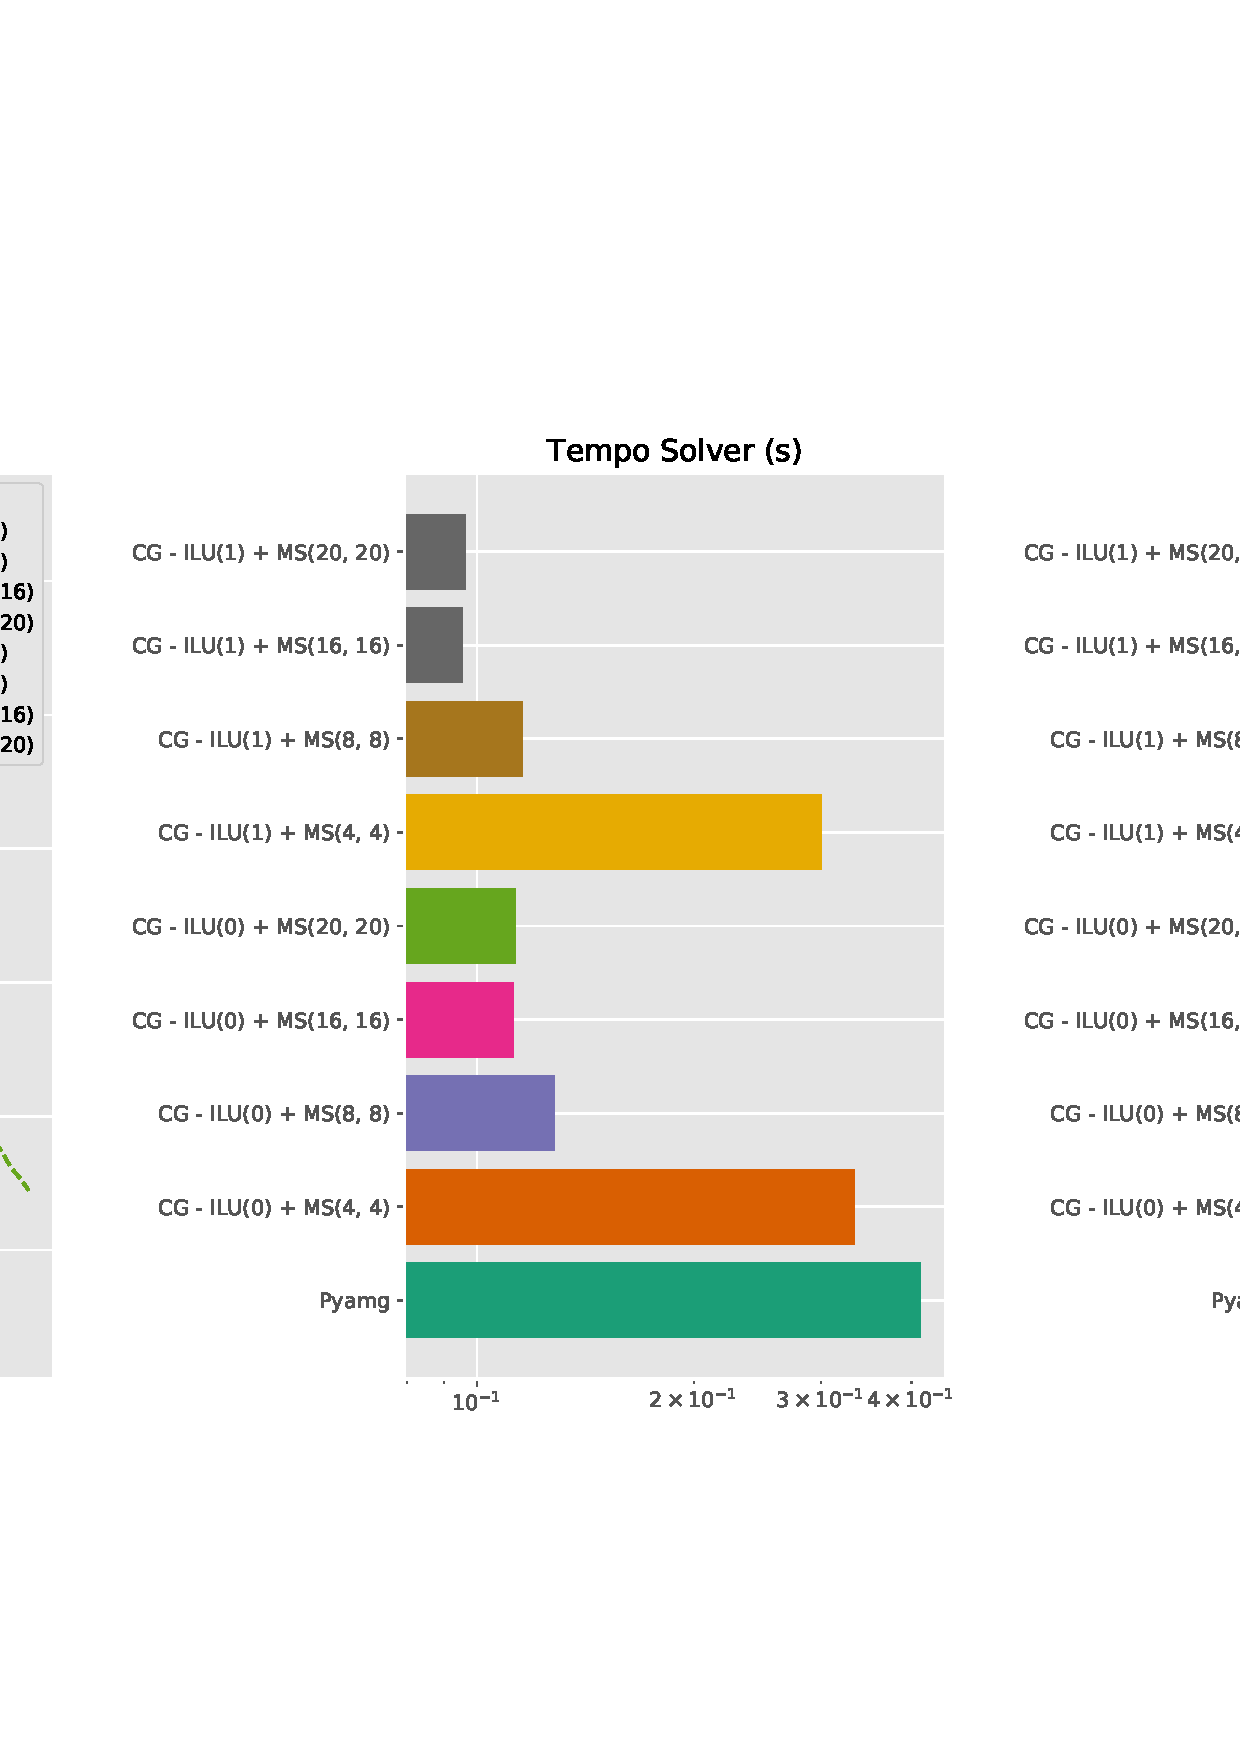
\includegraphics[width=\textwidth]{chap08/figs/reservatorio100x100_1.png}
\end{figure}

Um primeiro ponto a se observar no gráfico da esquerda é o aumento do número de iterações a cada vez que se aumenta o fator de engrossamento da malha. 
Isso ocorre pois a solução do problema grosso se torna cada vez mais distante da solução da malha fina fazendo com que o pré-condicionador funcione pior. 
Entretanto, quanto mais grossa a malha, mais fácil a solução sistema linear grosso e, portanto, existe uma solução de compromisso 
entre o engrossamento da malha e o tempo de execução. É importante lembrar também que sempre é necessário pagar o custo da multiplicação pelo
operador de prolongamento e de restrição que independe do nível de engrossamento, por conta disso, o tempo da iteração do engrossamento 16x16
é semelhante ao 20x20. No caso A, a solução de menor tempo é quando o nível grosso é construído ao se montar elementos grossos utilizando 16x16 elementos finos. 



Na figura \ref{fig:reservatorio100x100_2} é apresentado a comparação da solução do sistema utilizando o melhor método multiescala com o gradiente conjugado 
utilizando como precondicionador o ILU(0), ILU(1) e solver multigrid Pyamg. 
ode-se notar que apesar da redução de iterações dos método multiescala e do método multigrid, os pré-condicionadores ILU(0) e ILU(1) são mais eficientes na resolução do sistema. 


\begin{figure}[!htbp]
\caption{Resultados para caso A. Histórico do resíduo relativo ao longo das iterações, tempo do solver em segundos, número de iterações em função do fator de engrossamento da malha e tempo do solver por iteração. }
\label{fig:reservatorio100x100_2}
\centering
\includegraphics[width=\textwidth]{chap08/figs/reservatorio100x100_2.png}
\end{figure}


As figuras \ref{fig:reservatorio320x320_1} e \ref{fig:reservatorio320x320_2} apresentam os mesmos resultados para o caso B.
Nesse caso, o engrossamento multiescala de 20x20 é o que resolve o solver em menor tempo, conseguindo inclusive superar o tempo de solução com o solver pré-condicionador ILU(1).
O tempo de solução com MS+ILU(1) tem uma melhora de 11,4\% em relação ao tempo do ILU(0). Quando comparado MS+ILU(1) contra ILU(1) o tempo de execução é 45,7\% tempo menor.
Além disso, o Pyamg não conseguiu convergir para a solução do problema, parando a execução quando o resíduo atingiu a casa dos $10^{-3}$


\begin{figure}[!htbp]
\caption{Resultados para caso B. Histórico do resíduo relativo ao longo das iterações, tempo do solver em segundos, número de iterações em função do fator de engrossamento da malha e tempo do solver por iteração. }
\label{fig:reservatorio320x320_1}
\centering
\includegraphics[width=\textwidth]{chap08/figs/reservatorio320x320_1.png}
\end{figure}


\begin{figure}[!htbp]
\caption{Resultados para caso B. Histórico do resíduo relativo ao longo das iterações, tempo do solver em segundos, número de iterações em função do fator de engrossamento da malha e tempo do solver por iteração. }
\label{fig:reservatorio320x320_2}
\centering
\includegraphics[width=\textwidth]{chap08/figs/reservatorio320x320_2.png}
\end{figure}


A seguir são apresentados resultados para o corte dos modelos D e E respectivamente nas figuras \ref{fig:casoD_2} e \ref{fig:casoE_2}. 
São apresentadas apenas a comparação entre os pré-condicionadores multiescala, Pyamg, ILU(0) e ILU(1). 


A seguir, as figuras \ref{fig:casoC_2}, \ref{fig:casoD_2} e \ref{fig:casoE_2} apresentam os resultados para os casos C, D e E. 
Em todos os gráficos é mostrado apenas o pré-condicionador multiescala que obteve o melhor desempenho entre os fatores de engrossamento de 2x2, 4x4, 8x8, 16x16, 32x32.


% \begin{figure}[!htbp]
% \label{fig:casoD_1}
% \centering
% \includegraphics[width=\textwidth]{chap08/figs/casoD_1.png}
% \caption{Resultados para caso D. Histórico do resíduo relativo ao longo das iterações, tempo do solver em segundos, número de iterações em função do fator de engrossamento da malha e tempo do solver por iteração. }
% \end{figure}

\begin{figure}[!htbp]
\caption{Comparação entre multiescala, multigrid e pré-condicionador ILU para o caso D. Histórico do resíduo relativo ao longo das iterações, tempo do solver em segundos e tempo do solver por iteração. }
\label{fig:casoD_2}
\centering
\includegraphics[width=\textwidth]{chap08/figs/casoD_2.png}
\end{figure}

    
\begin{figure}[!htbp]
\caption{Comparação entre multiescala, multigrid e pré-condicionador ILU para o caso D. Histórico do resíduo relativo ao longo das iterações, tempo do solver em segundos e tempo do solver por iteração. }
\label{fig:casoE_2}
\centering
\includegraphics[width=\textwidth]{chap08/figs/casoE_2.png}
\end{figure}


\subsection{Acurácia da solução grossa}

Nos resultados mostrados nas seções anteriores, era utilizado um solver direto para resolver 
o sistema grosso. Em casos que a malha foi suficientemente reduzida esse tempo de solução é desprezível,
porém, para casos o fator de engrossamento é pequeno resolver exatamente o nível grosso aumenta
o tempo de execução (por exemplo, o caso ILU(1) + MS(4,4) em \ref{fig:reservatorio100x100_1}). 
Além disso, caso modelos muito refinados sejam utilizados o espaço grosseiro pode continuar
grande e precise ser resolvido com métodos iterativos, como por exemplo para soluções de casos
com centenas de milhões de elementos como o mostrado em \cite{geomecrio}.


A avaliação foi feita da seguinte maneira: foi avaliada a quantidade de iterações para resolver o sistema linear com tolerância de $10{-6}$ utilizando o pré-condicionador multiescala com solver do espaço grosso um gradiente conjugado com tolerância variando de $10^{-10}$  a $10^{-1}$. 

  \chapter{Conclusão e Trabalhos Futuros} \label{ch:conclusoes}
  
Essa dissertação apresentou a teoria necessária para a construção de um simulador de geomecânica elástico utilizando o método dos elementos finitos e método multiescala como pré-condicionador para sistemas lineares. Como resultados foram apresentadas comparações entre a abordagem de combinar pré-condicionadores de forma aditiva e multiplicativa que mostram que, para fatores de engrossamento grandes o suficientes, pode-se obter soluções em torno de 10\% a 15\%  mais rápidas utilizando o pré-condicionador aditivo. Além disso, foram apresentadas comparações utilizando o método do gradiente conjugado com pré-condicionador  multiescala, ILU e multigrid para modelos sintéticos e também para casos reais. A comparação entre o multiescala e o ILU mostrou que o primeiro reduz o número de iterações e encontra soluções mais rapidamente que o ILU mostrando speed-ups de até 3,8 vezes. A comparação entre o multigrid e multiescala mostrou que apenas no caso E o multigrid realizou mais iterações enquanto que nos outros a quantidade de iterações foi similar. Porém, com relação a métrica do número de operações realizadas as relaxações dos vários níveis do multigrid  tem um custo bem maior por iteração, tornando o multiescala uma opção mais atrativa.  Outro ponto importante é que os resultados mostraram também a eficácia do método para a simulação de modelos com dados reais de campos que possuem propriedades heterogêneas e grids mais complexos. 
%É possível ver também que na simulações dos casos D e E o multigrid começa com uma inclinação elevada na redução do resíduo e a partir de certo ponto a inclinação muda para uma redução menor do resíduo, enquanto que a inclinação do método multiescala permanece mais constante. Uma possível tentativa para atingir reduções elevadas no resíduo nas primeiras iterações do método multiescala é a utilização do método multiescala multi-nível.

Visto o bom resultado do método para os sistemas lineares geomecânicos, uma implementação paralela e algébrica tem grandes possibilidades de reduzir o tempo de simulação em modelos de simulação geomecânica em três dimensões. Além disso, como o operador multiescala também possui uma dimensão bem menor que a do operador do grid original, ele pode ser pensando com um pré-condicionador grosseiro geral de todo o modelo resolvendo dessa forma o problema do aumento do número de partições quanto mais o domínio é dividido. Com essas ideias pode-se melhorar ainda mais os resultados obtidos em \citet{geomecrio} tornando as execuções do simulador geomecânico da Petrobras ainda mais rápidas. Essas novas implementações tem diversos desafios em relação ao paralelismo como a coordenação da solução dos problemas locais em paralelo, implementação de produtos matriz-matriz esparsas para  cálculo do operador grosso, comunicação dos resultados de problemas locais nas fronteiras do processos, dentre outros.



  
  \backmatter
  \bibliographystyle{coppe-unsrt}
  \bibliography{thesis}

  \appendix
  
  
\if\realreservoir1
  \include{append/appendA}
\fi


  \chapter{Configurações de solver utilizadas pelo Pyamg} \label{ch:pyamgSolver}


Seguem abaixo as chamadas com os parâmetros para construção dos solvers multigrid  utilizados pelo PyAMG para os resultados apresentados no Capítulo \ref{ch:resultados}. Esses foram retornados pelo script \textbf{solver\_diagnostics.py}. Em todos os casos a chamada do solver multigrid foi sugerida com o ciclo W e como pré-condicionador para o Gradiente Conjugado. 


\subsubsection{Caso A e Caso B}

\begin{lstlisting}[
    basicstyle=\small, %or \small or \footnotesize etc.
]
smoothed_aggregation_solver(A, B=B, BH=BH,
  strength=('evolution', {'k': 2, 'proj_type': 'l2', 'epsilon': 2.0}),
  smooth=('energy', {'krylov': 'cg', 'maxiter': 2, 
          'degree': 1, 'weighting': 'local'}),
  improve_candidates=[('block_gauss_seidel', 
                      {'sweep': 'symmetric', 'iterations': 4}), 
                      None, None, None, None, None, None,
                      None, None, None, None, None,
                      None, None, None],
  aggregate="standard",
  presmoother=('block_gauss_seidel', 
               {'sweep': 'symmetric', 'iterations': 1}),
  postsmoother=('block_gauss_seidel', 
                {'sweep': 'symmetric', 'iterations': 1}),
  max_levels=15,
  max_coarse=300,
  coarse_solver="pinv")
\end{lstlisting}

\subsubsection{Caso C}

\begin{lstlisting}[
    basicstyle=\small, %or \small or \footnotesize etc.
]
smoothed_aggregation_solver(A, B=B, BH=BH,
  strength=('evolution', {'k': 2, 'proj_type': 'l2', 'epsilon': 2.0}),
  smooth=('energy', {'krylov': 'cg', 'maxiter': 2, 
                     'degree': 1, 'weighting': 'local'}),
  improve_candidates=[('block_gauss_seidel', 
                      {'sweep': 'symmetric', 'iterations': 4}), 
                      None, None, None, None, None, None, None, 
                      None, None, None, None, None, None, None],
  aggregate="standard",
  presmoother=('block_gauss_seidel', 
               {'sweep': 'symmetric', 'iterations': 1}),
  postsmoother=('block_gauss_seidel', 
                {'sweep': 'symmetric', 'iterations': 1}),
  max_levels=15,
  max_coarse=300,
  coarse_solver="pinv")
\end{lstlisting}


\subsubsection{Caso D e Caso E}

\begin{lstlisting}[
    basicstyle=\small, %or \small or \footnotesize etc.
]
smoothed_aggregation_solver(A, B=B, BH=BH,
  strength=('evolution', {'k': 2, 'proj_type': 'l2', 'epsilon': 2.0}),
  smooth=('energy', {'krylov': 'cg', 'maxiter': 2, 
                     'degree': 1, 'weighting': 'local'}),
  improve_candidates=None,
  aggregate="standard",
  presmoother=('block_gauss_seidel', 
               {'sweep': 'symmetric', 'iterations': 1}),
  postsmoother=('block_gauss_seidel', 
                {'sweep': 'symmetric', 'iterations': 1}),
  max_levels=15,
  max_coarse=300,
  coarse_solver="pinv")
\end{lstlisting}
  



\end{document}
